% Page style for this chapter
	\pagestyle{fancy}
	\lhead{{\sffamily \MakeUppercase{6. Validation}}}
	\chead{}
	\rhead{{\sffamily \MakeUppercase\rightmark}}
	\lfoot{}
	\cfoot{{\sffamily \thepage}}
	\rfoot{}

\chapter{Validation of the Guinea Pig Model}
\label{sect:validation}

% Textbox
\begin{center}
	\begin{tcolorbox}[title=\boxtitle]
		\begin{itemize}[leftmargin=*,labelindent=2ex,labelsep=1.5ex,itemsep=0pt,parsep=0pt]
			\item How realistic are the model predictions?
			\item How sensitive is the model to various input parameters?
			\item What is the set of ideal inputs?
		\end{itemize}
	\end{tcolorbox}
\end{center}


\section{Introduction}
\label{sect:validation_intro}

\textit{This chapter is based on the paper by Wong~\etal~\cite{wong2016}, which
has been published in IEEE Transactions on Biomedical Engineering.}

Experimental verification of a model is always necessary \cite{miller1990,
schimpf1998}. Computational models capture the physics of the system from a
theoretical, bottom-up approach, so there are a number of simplifying
assumptions and potential errors inherent to the modelling process that can
affect the accuracy of the \insilico~results. In the cochlear implant (CI)
research community, there is already a reluctance to trust the findings from
existing computational models. This is probably due to a range of factors,
including the crude geometry of some existing volume conduction models (VCMs),
unfamiliarity with computational methods, insufficient justification of
assumptions, and the limited ability of models to predict psychophysical
outcomes with consistent accuracy. Validation is therefore an essential step to
pursue before the model is used for any further investigations.

% Parameters must be controlled in order to replicate the in vivo situation as
% closely as possible. Of the four inputs described in \S\ref{sect:inputs}, only
% the electrical load is well controlled, since the injected current pulse is
% managed by the pre-programmed stimulator electronics.

% What about the use of EIT, MREIT? Probably not that useful here.

The primary goal of this chapter is to compare the \insilico{} predictions of
the guinea pig model against similar \invivo{} voltage tomography data obtained
independently at the Bionics Institute in Melbourne, Australia by Shefin George
(under the supervision of James Fallon). This will help to determine whether or
not the model outputs are reasonable. If a good correlation between the
\insilico{} and \invivo{} results is found, confidence in the model will be
established, and some of the concerns surrounding the use of VCMs may be
alleviated.

The correlation is expected to be strong because the new model includes several
improvements over previous models. Existing VCMs typically use histological
sections traced and swept along a spiral path, or a simplified computer-aided
design (CAD) geometry. This model was reconstructed from a stack of scanning
thin-sheet laser imaging microscopy (sTSLIM) images~\cite{santi2011}, so the
geometry is considerably more realistic: the hook region is accurately
represented and includes the round window membrane and the stapes; the scala
tympani and scala vestibuli are truly continuous at the helicotrema; the major
blood vessels and cerebrospinal fluid (CSF) in the modiolus were
incorporated---unique for VCMs of the cochlea. Furthermore, bone was not treated
as a homogeneous material, but instead separated into the modiolar bone, the
otic capsule, and the temporal bone. These have markedly different
microstructures and hence different electrical resistivities, so they should be
treated as separate material
domains~\cite{spelman1987,suesserman1992,micco2006,wong2013mb}.

The secondary goal of this chapter is to evaluate the validity of long-held
assumptions on material properties and boundary conditions. These two factors
are important in determining the \insilico{} results for any particular
geometry. An updated set of boundary conditions was tested relative to
Chapter~\ref{sect:boundary_conditions}, and the basic neural response was also
considered using the activating function (AF)~\cite{rattay1986}.

Like previous studies, this model assumes that the cochlear tissues are purely
resistive, based on the evidence provided by Spelman~\cite{spelman1982}.
Resistivity values from the literature (Table~\ref{table:gp_domains}) are used
as base values. There are no measurements in the literature for the round window
membrane, which is being incorporated into a VCM for the first time. To
determine the impact of any measurement uncertainties, as well as natural
variations in properties between individuals, the sensitivity of the model to
each tissue resistivity value was evaluated.

Boundary conditions are modeling constraints necessary for solving the field
problem~\cite{johnson2006} and should ideally replicate the physics at the
boundary of the modelled domain accurately. This is problematic for VCMs of the
cochlea simulating monopolar (MP) stimulation because the return electrode lies
outside the physical domain of the model. Existing models deal with this issue
by assuming that the end of the auditory nerve is
grounded~\cite{girzon1987,whiten2007}, that the ground is infinitely far
away~\cite{frijns2000}, or that boundary box surfaces are
grounded~\cite{rattay2001model,saba2012}---none of these perfectly match the
\invivo{} situation. Alternatively, they avoid the MP situation altogether and
focus on pseudo-monopolar or bipolar stimulation
~\cite{finley1990,frijns1995,hanekom2001,choi2004}. Although the simulation
results in these cases are indicative, they are less clinically relevant given
the widespread use of MP stimulation in CI recipients. To clarify how the
boundary condition assumption affects simulation results, several different
cases, reflecting the range of existing choices as well as more realistic
alternatives, are compared to provide some guidance for future modeling efforts.

\section{Method}

\textit{The following sections cover the procedures specific to performing the
validation study. For details about how the model was reconstructed from the
raw image stack and meshed, refer to \S{\ref{sect:method_gp}}.}

\subsection{\textit{In silico} Modelling}

A base case was first defined as a reference for comparison of the \insilico{}
results. All tissue domains were configured with isotropic resistivities as
in Table~\ref{table:gp_domains}. A 1~mA constant current source was placed at
the inner surface of the stimulating electrode, identical to that used for the
\invivo{} measurements. The external surface of the round window membrane was
insulated to prohibit current flow from the scala tympani into the
non-conductive middle ear air space, as expected \invivo{}. Lastly, the temporal
bone surface was grounded to represent the expected MP current sink.

A convergence test was then performed to ensure sufficient discretisation. Five
meshes were generated by varying the element size limits described in
\S\ref{sect:gp_mesh_gen}, then imported into COMSOL Multiphysics using the
NASTRAN file format. Both the PARDISO (direct) and Conjugate Gradient
(iterative) solvers were tested, with no observed difference in numerical
results. PARDISO just exceeded the computer's RAM capacity when solving
quadratically discretised meshes, so the Conjugate Gradient solver was used to
prevent writing to disk.

Using the converged mesh, both material properties and boundary conditions were
altered \textit{ceteris paribus} from the base case. For the sensitivity
analysis on material properties, individual tissue resistivities were set to
either double or half of the base value (\`a la Finley~\cite{finley1989} and
Rattay~\cite{rattay2001model}), or the highest or lowest values from literature,
whichever deviated more from the base value. Since there was no data for the
round window membrane, its resistivity was assumed to be 1000~$ \Omega \cdot $m
based on the geometric average of Reissner's membrane and the basilar membrane
(see Table~\ref{table:gp_domains}), and an order of magnitude variation was
tested to account for the additional uncertainty.

For the boundary condition tests, the base case rerun with each of the
following boundary conditions:
\begin{enumerate}[after=\vspace{1.5\medskipamount}]
	\item Ground the auditory nerve trunk only;
	\item Ground the caudal aspect of the temporal bone surface;
	\item Ground the entire temporal bone surface;
	\item Apply a voltage offset on the temporal bone surface;
	\item Ground the entire outer surface of the surrounding sphere;
	\item Ground at an infinite large surrounding sphere.
\end{enumerate}

The corresponding boundary surfaces are shown in
Figure~\ref{fig:boundary_surfaces}. Boundary conditions 2--5 were applied on a
surrounding sphere of radius 5~mm because this size was found to be sufficiently
large for replicating far-field effects~\cite{wong2013ciap}. For grounding at
infinity, a second shell of radius 8~mm was added and configured as an infinite
element domain in COMSOL, with resistivity set to that of the guinea pig
skull~\cite{suesserman1992}.

\begin{figure}
	\centering
	
	\begin{subfigure}[t]{0.4\textwidth}
        \centering
        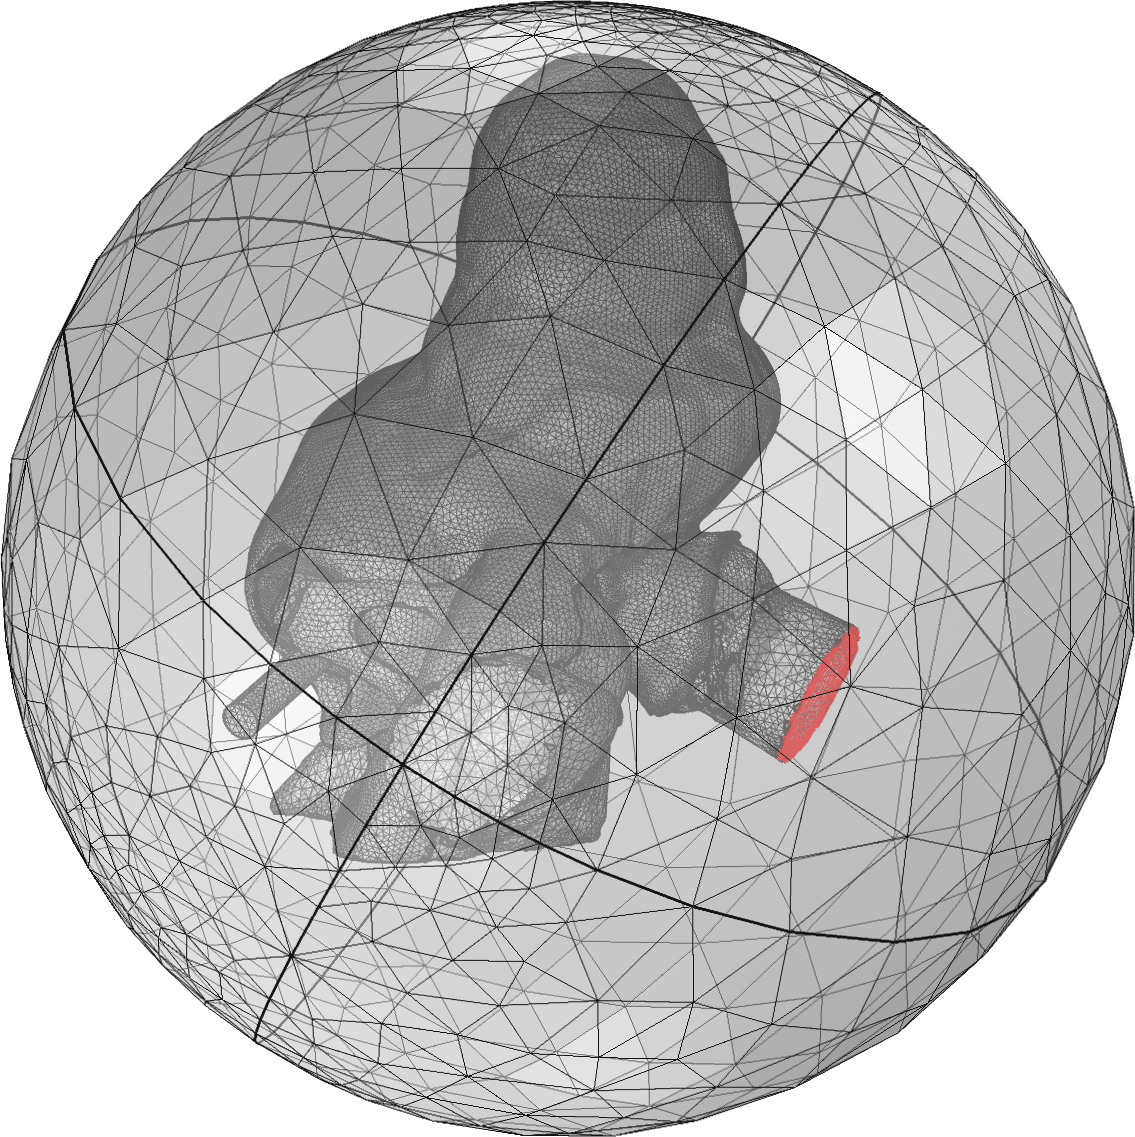
\includegraphics[height=4.5cm]{Validation/mesh_nerve}
        \caption{}
        \label{fig:mesh_nerve}
    \end{subfigure}%
	\begin{subfigure}[t]{0.4\textwidth}
        \centering
        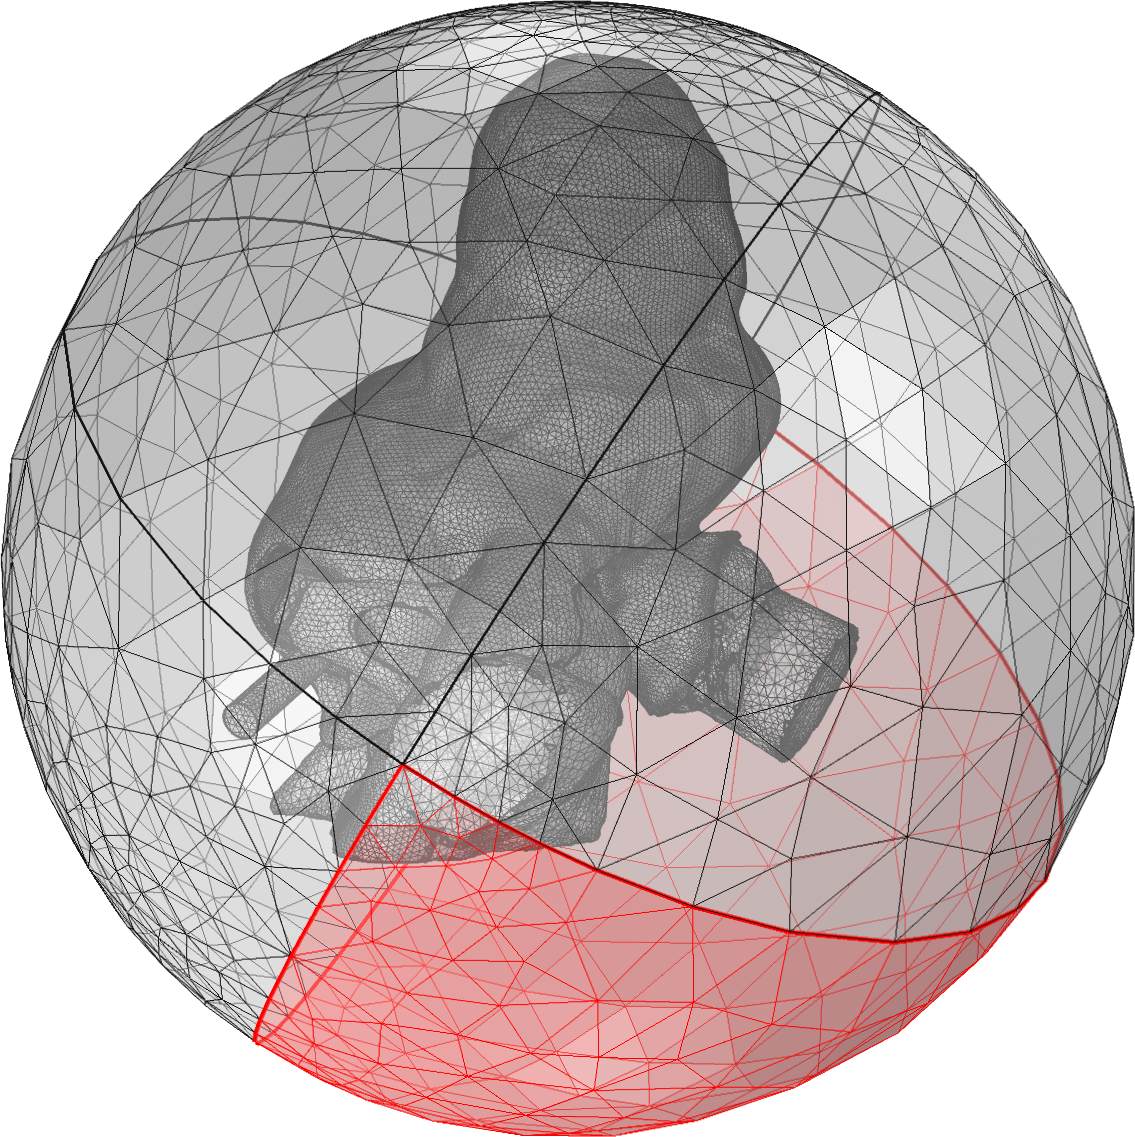
\includegraphics[height=4.5cm]{Validation/mesh_caudal}
        \caption{}
        \label{mesh_caudal}
    \end{subfigure}\\%
    \vspace{1em}%
	\begin{subfigure}[t]{0.4\textwidth}
        \centering
        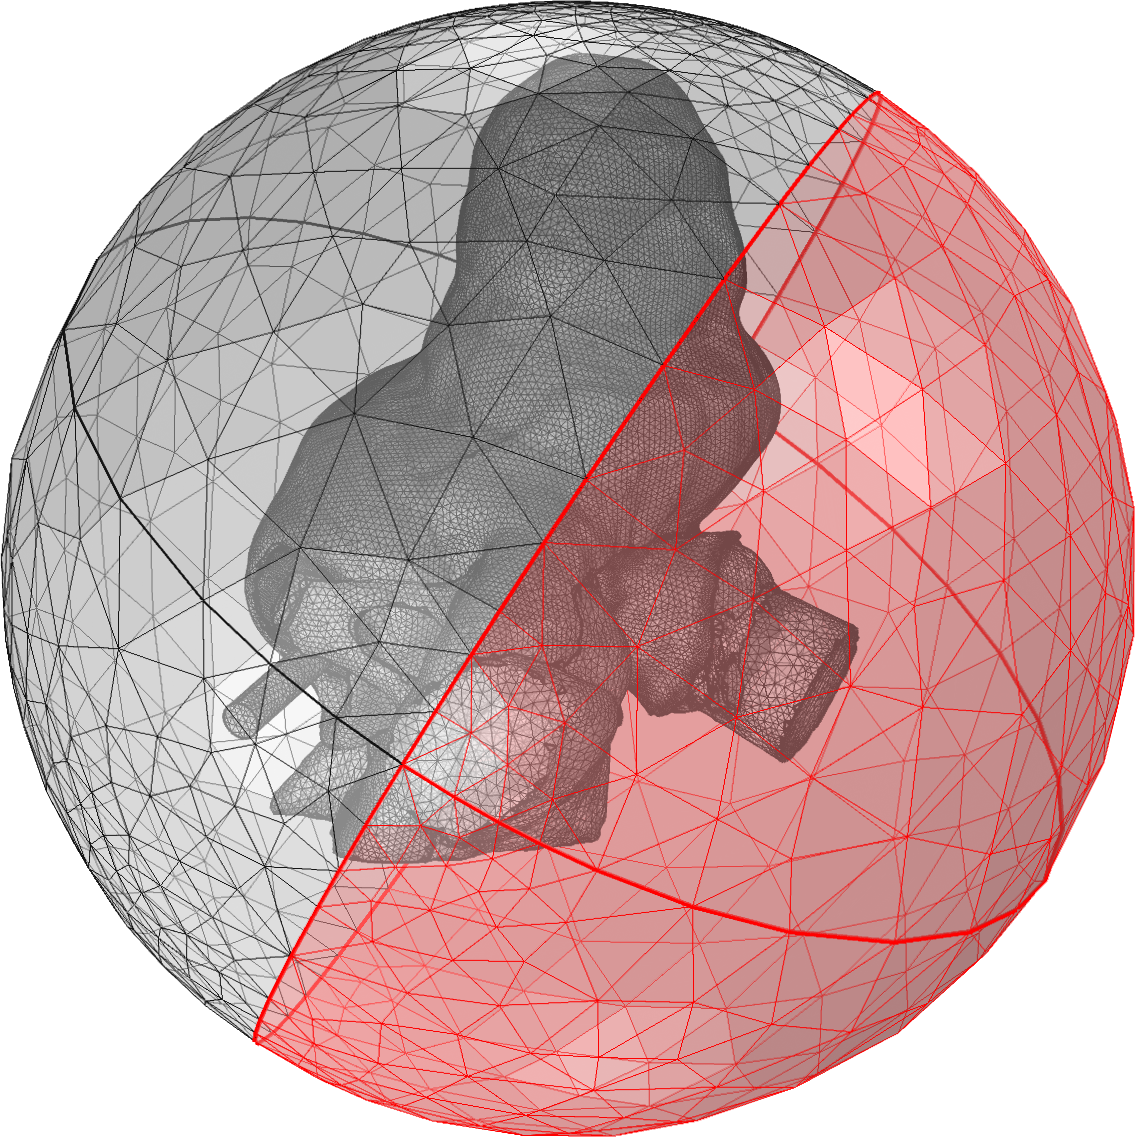
\includegraphics[height=4.5cm]{Validation/mesh_hemi}
        \caption{}
        \label{mesh_hemi}
    \end{subfigure}%
	\begin{subfigure}[t]{0.4\textwidth}
        \centering
        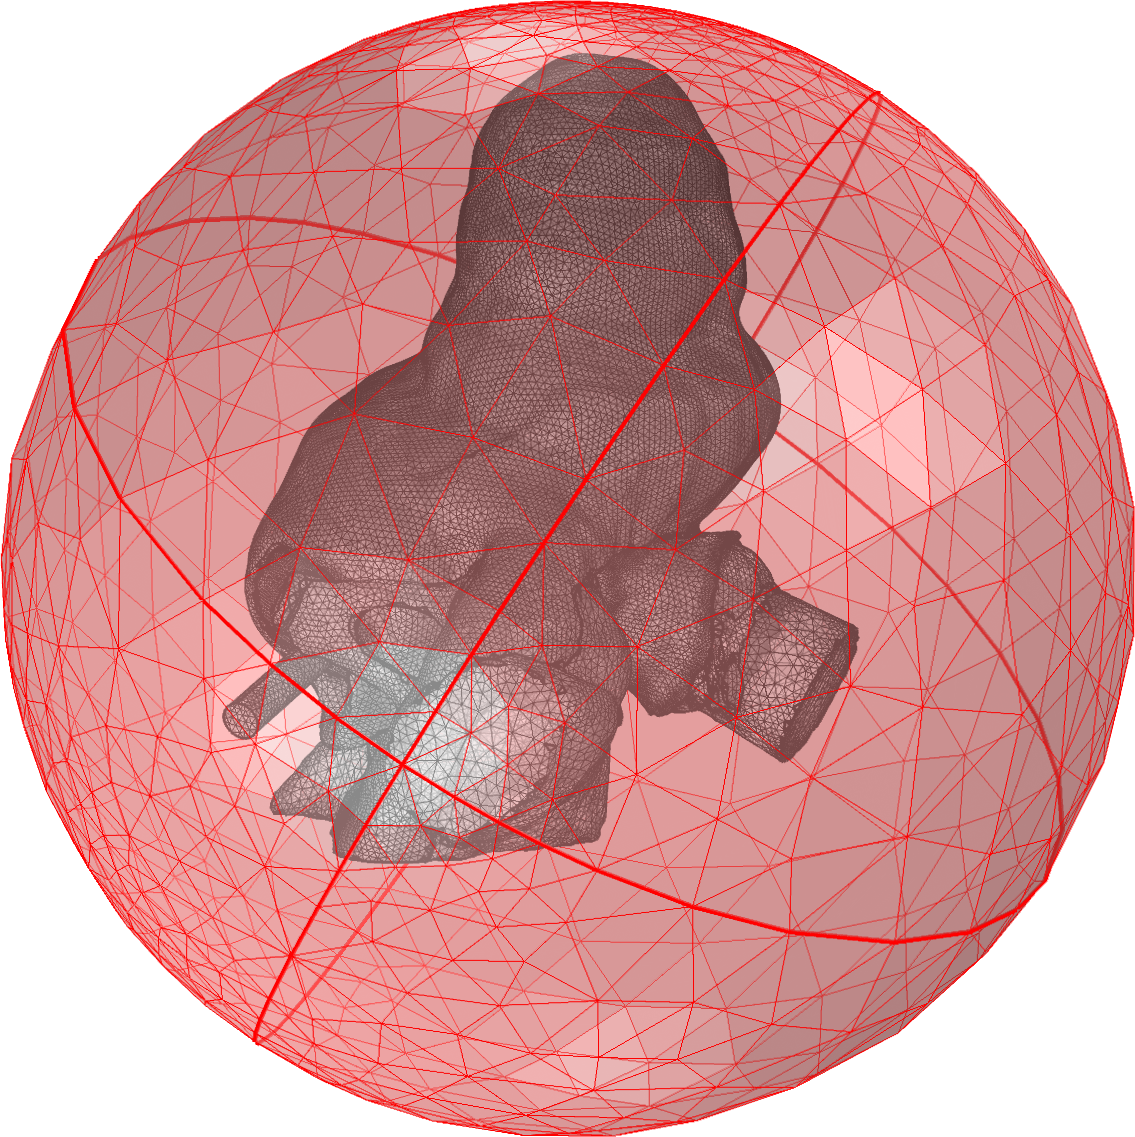
\includegraphics[height=4.5cm]{Validation/mesh_sph}
        \caption{}
        \label{mesh_sph}
    \end{subfigure}\\%
	\vspace{1em}%
	\begin{subfigure}[t]{0.5\textwidth}
        \centering
        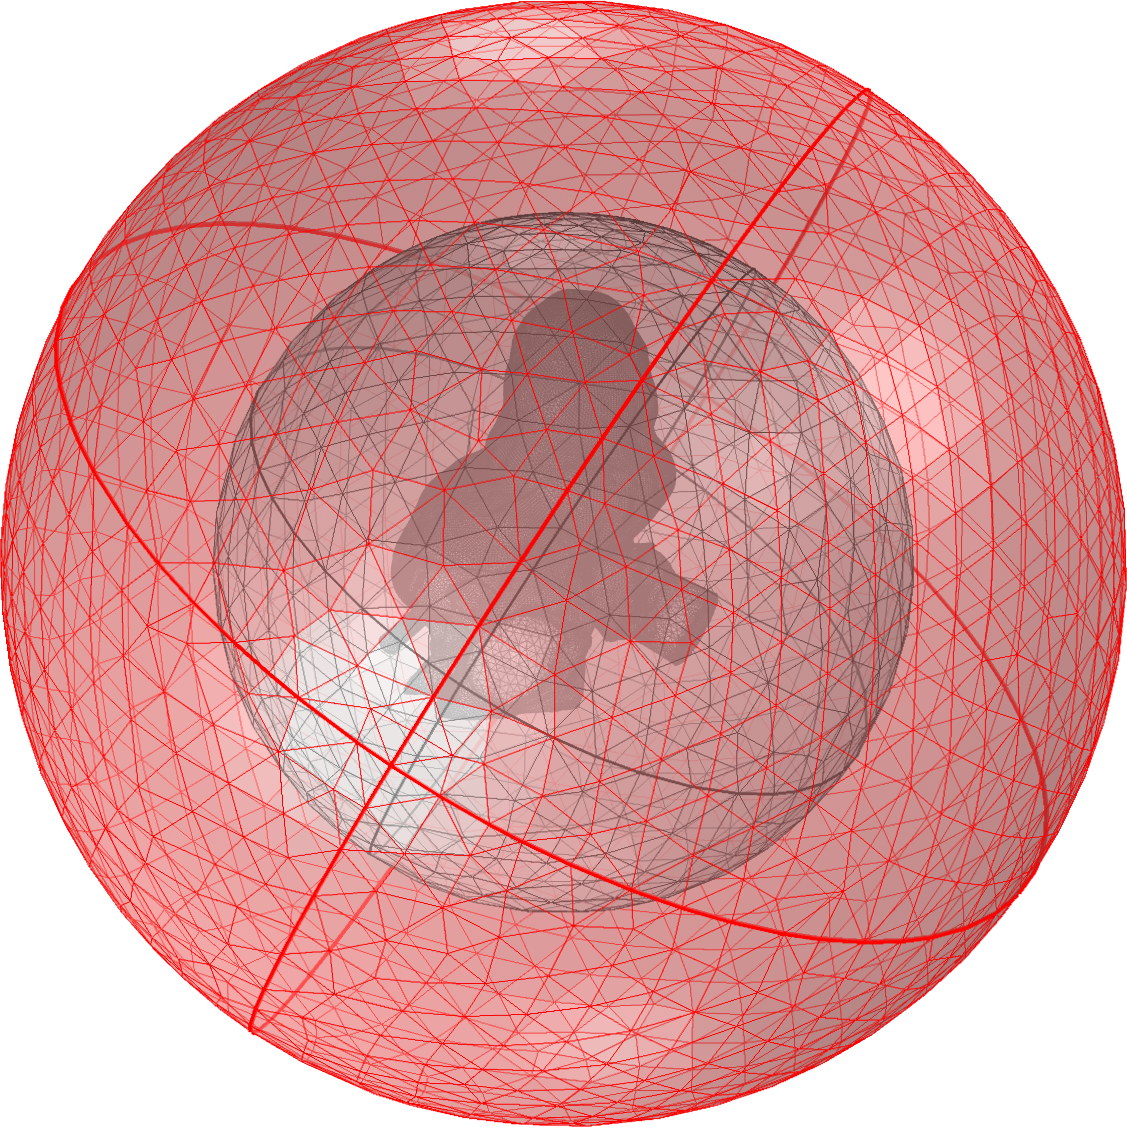
\includegraphics[height=7.5cm]{Validation/mesh_inf}
        \caption{}
        \label{mesh_inf}
    \end{subfigure}%
    
    \caption[Surface selections for boundary conditions]{Surface selections for
	boundary conditions: (a) the end of the auditory nerve trunk; (b) caudal aspect
	of the temporal bone surface; (c) the temporal bone surface; (d) the surrounding
	sphere; (e) at infinity. The outermost domain in (e) is configured as an
	infinite element domain.}
	\label{fig:boundary_surfaces}
\end{figure}

The voltage offset boundary condition is a novel proposal. In a real CI
recipient, the stimulating current must pass through the cochlear tissues as
well as the rest of the head in order to reach the return electrode under MP
stimulation (see Figure~\ref{fig:voltage_divider}). If the resistance of the
head is not accounted for in the model, the total resistance will be
underestimated. The circuit is also a voltage divider, so given the non-zero
resistance of the head, the electric potential at the model boundary should also
be non-zero (i.e. not grounded). The offset value for these simulations was
determined as the average difference in terminal voltages between grounding at
the temporal bone surface and the mean \invivo{} profile.

\begin{figure}
	\centering
	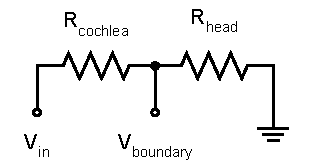
\includegraphics[height=3.2cm]{Validation/voltage_divider}
	\caption[Equivalent circuit for the entire head]{The modelled domain
	only includes the resistance inside the cochlea. For monopolar stimulation,
	injected current must also overcome the resistance of the head in order to reach
	the ground electrode. This acts like a voltage divider, so the electric
	potential at the model boundary should be non-zero. (Copyright \textcopyright{}
	2015, IEEE.)}
	\label{fig:voltage_divider}
\end{figure}

The primary model output was the average voltage at each electrode, because this
could be directly compared with the \invivo{} results. The magnitude and
direction of current flow were depicted using streamline plots of current
density seeded on a regular quadratic grid over the surface of the active
electrode (see Appendix~\ref{appendix:streamline_seeding}). Neuron trajectories
covering the first 570 degrees of the cochlea were modelled in MATLAB by
connecting key points from the tips of the peripheral processes, through the
cross-sectional center of the spiral ganglion, and down along the cochlear nerve
trunk (see Figure~\ref{fig:fibre_trajectories}), similar to
Kalkman~\etal~\cite{kalkman2014}. For each neuron, nodes of Ranvier were placed
at fixed intervals from the point in Rosenthal's canal. Spacing resembled that
used in the GSEF neural model~\cite{frijns1995}: 175~$ \upmu $m along the
peripheral process and 300~$ \upmu $m along the axon. The AF, i.e. the discrete
second derivative of electric potential with respect to distance along the
fiber~\cite{reilly1998}, was computed for each set of adjacent nodal triads
along 100 equally spaced fibers, then plotted along the unrolled neural sheet
(Figure~\ref{fig:unroll_neural_sheet}). This signifies the degree to which the
underlying electrophysiological requirements for neural firing are met.

\begin{figure}
	\centering
	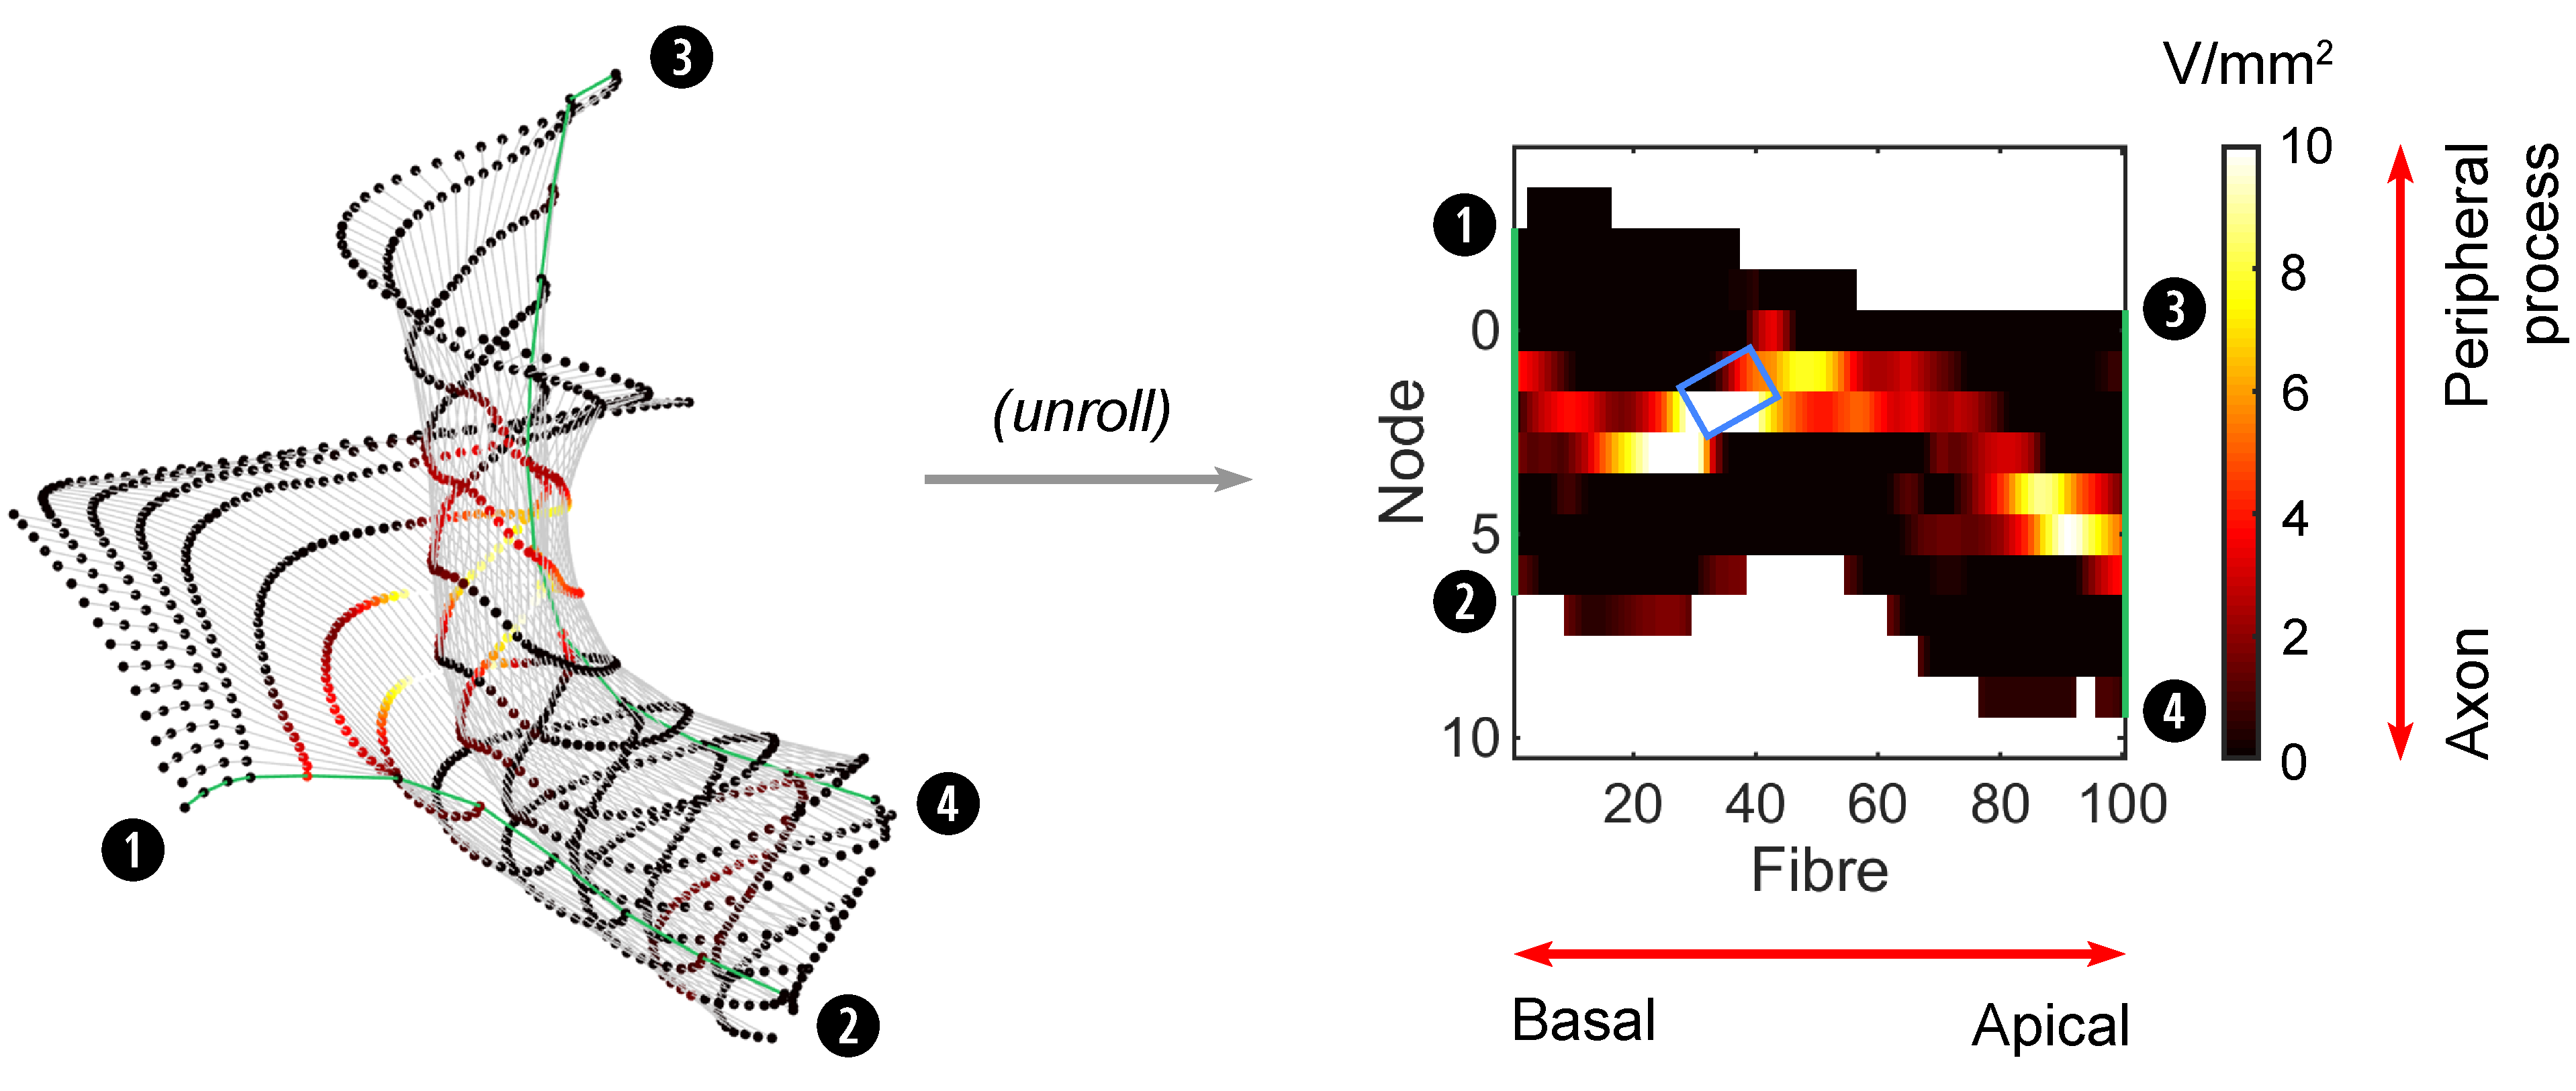
\includegraphics[width=14.5cm]{Validation/unroll_neural_sheet}
	\caption[Unrolling the neural sheet for 2D activating function plots]{Unrolling
	the neural sheet for 2D activating function plots. The data shown here are for
	the base case scenario. The coordinate system follows that of
	Kalkman~\etal~\cite{kalkman2014}, but here Rosenthal's canal is always at
	node 0. Fibres 1 and 100 are traced in green, and the blue box in the 2D plot
	marks the approximate location of the stimulating electrode (E4). (Copyright
	\textcopyright{} 2015, IEEE.)}
	\label{fig:unroll_neural_sheet}
\end{figure}

\subsection{\textit{In vivo} Measurements}

Voltage tomography measurements were collected from eight (N=8) adult pigmented
guinea pigs (500--800~g) for comparison with the \insilico{} results. All
procedures were approved by the Royal Victorian Eye and Ear Hospital Animal
Research and Ethics Committee (project number 12/250AB, granted 28 February
2012; see Appendix~\ref{appendix:ethics}) and were in accordance with the
Australian Code of Practice for the Care and Use of Animals for Scientific
Purposes. All procedures were performed in an electrically isolated Faraday
room.

The animals were anaesthetised using isoflurane (1.5--2\%) and oxygen (1~L/min).
Respiration rate (normal levels: 15--25~breaths/min) and end-tidal \ce{CO2}
levels (normal levels: 1--3\%) were monitored over the duration of the
experiment (2--3~hours). Core body temperature was maintained at $ 37.0 \pm 1
^{\circ} $C. A post-auricular incision was made and the left cochlea was
surgically exposed. Each animal was implanted with a Hybrid-L8 (HL8) array,
containing eight intracochlear platinum half-band electrodes on a silicone
carrier. The electrode array was inserted approximately 6~mm through the round
window into the scala tympani, typically placing 7--8 electrodes within the
scala. A platinum ball electrode placed in the neck muscles served as the MP
return and reference electrode.

For each intracochlear electrode, a monopolar cathodic-first biphasic pulse
(25~$ \upmu $s per phase and 8~$ \upmu $s inter-phase gap) was delivered with an
amplitude of 1~mA. The voltage at each of the non-stimulating electrodes was
measured with respect to the reference electrode at the end of the cathodic
phase. The voltage at the stimulating electrode was estimated as the maximum
among the values extrapolated from all available adjacent pairs, as adapted from
van den Honert and Kelsall~\cite{vandenhonert2007}, to ensure that the sharpness
of the current spread function was not underestimated.

\section{Results}

\subsection{\textit{In vivo} Data}

The raw measurements for all eight guinea pigs during stimulation at E4 are
shown in Figure~\ref{fig:in_vivo_data}. (Only results at E4 are presented for
brevity.) Differences between guinea pigs were observed, presumably due to the
unique geometry of each cochlea and its surrounding tissues, variations in the
surgical insertion of the implants and the resistivity of the tissues, and other
subject-specific factors. Most of the profiles clustered around the average, so
a mean profile was calculated to serve as a benchmark for comparison with the
\insilico{} results. The minimum to maximum voltage range over all specimens was
also found and is shaded in Figure~\ref{fig:in_vivo_data}.

\begin{figure}[p]
	\centering
	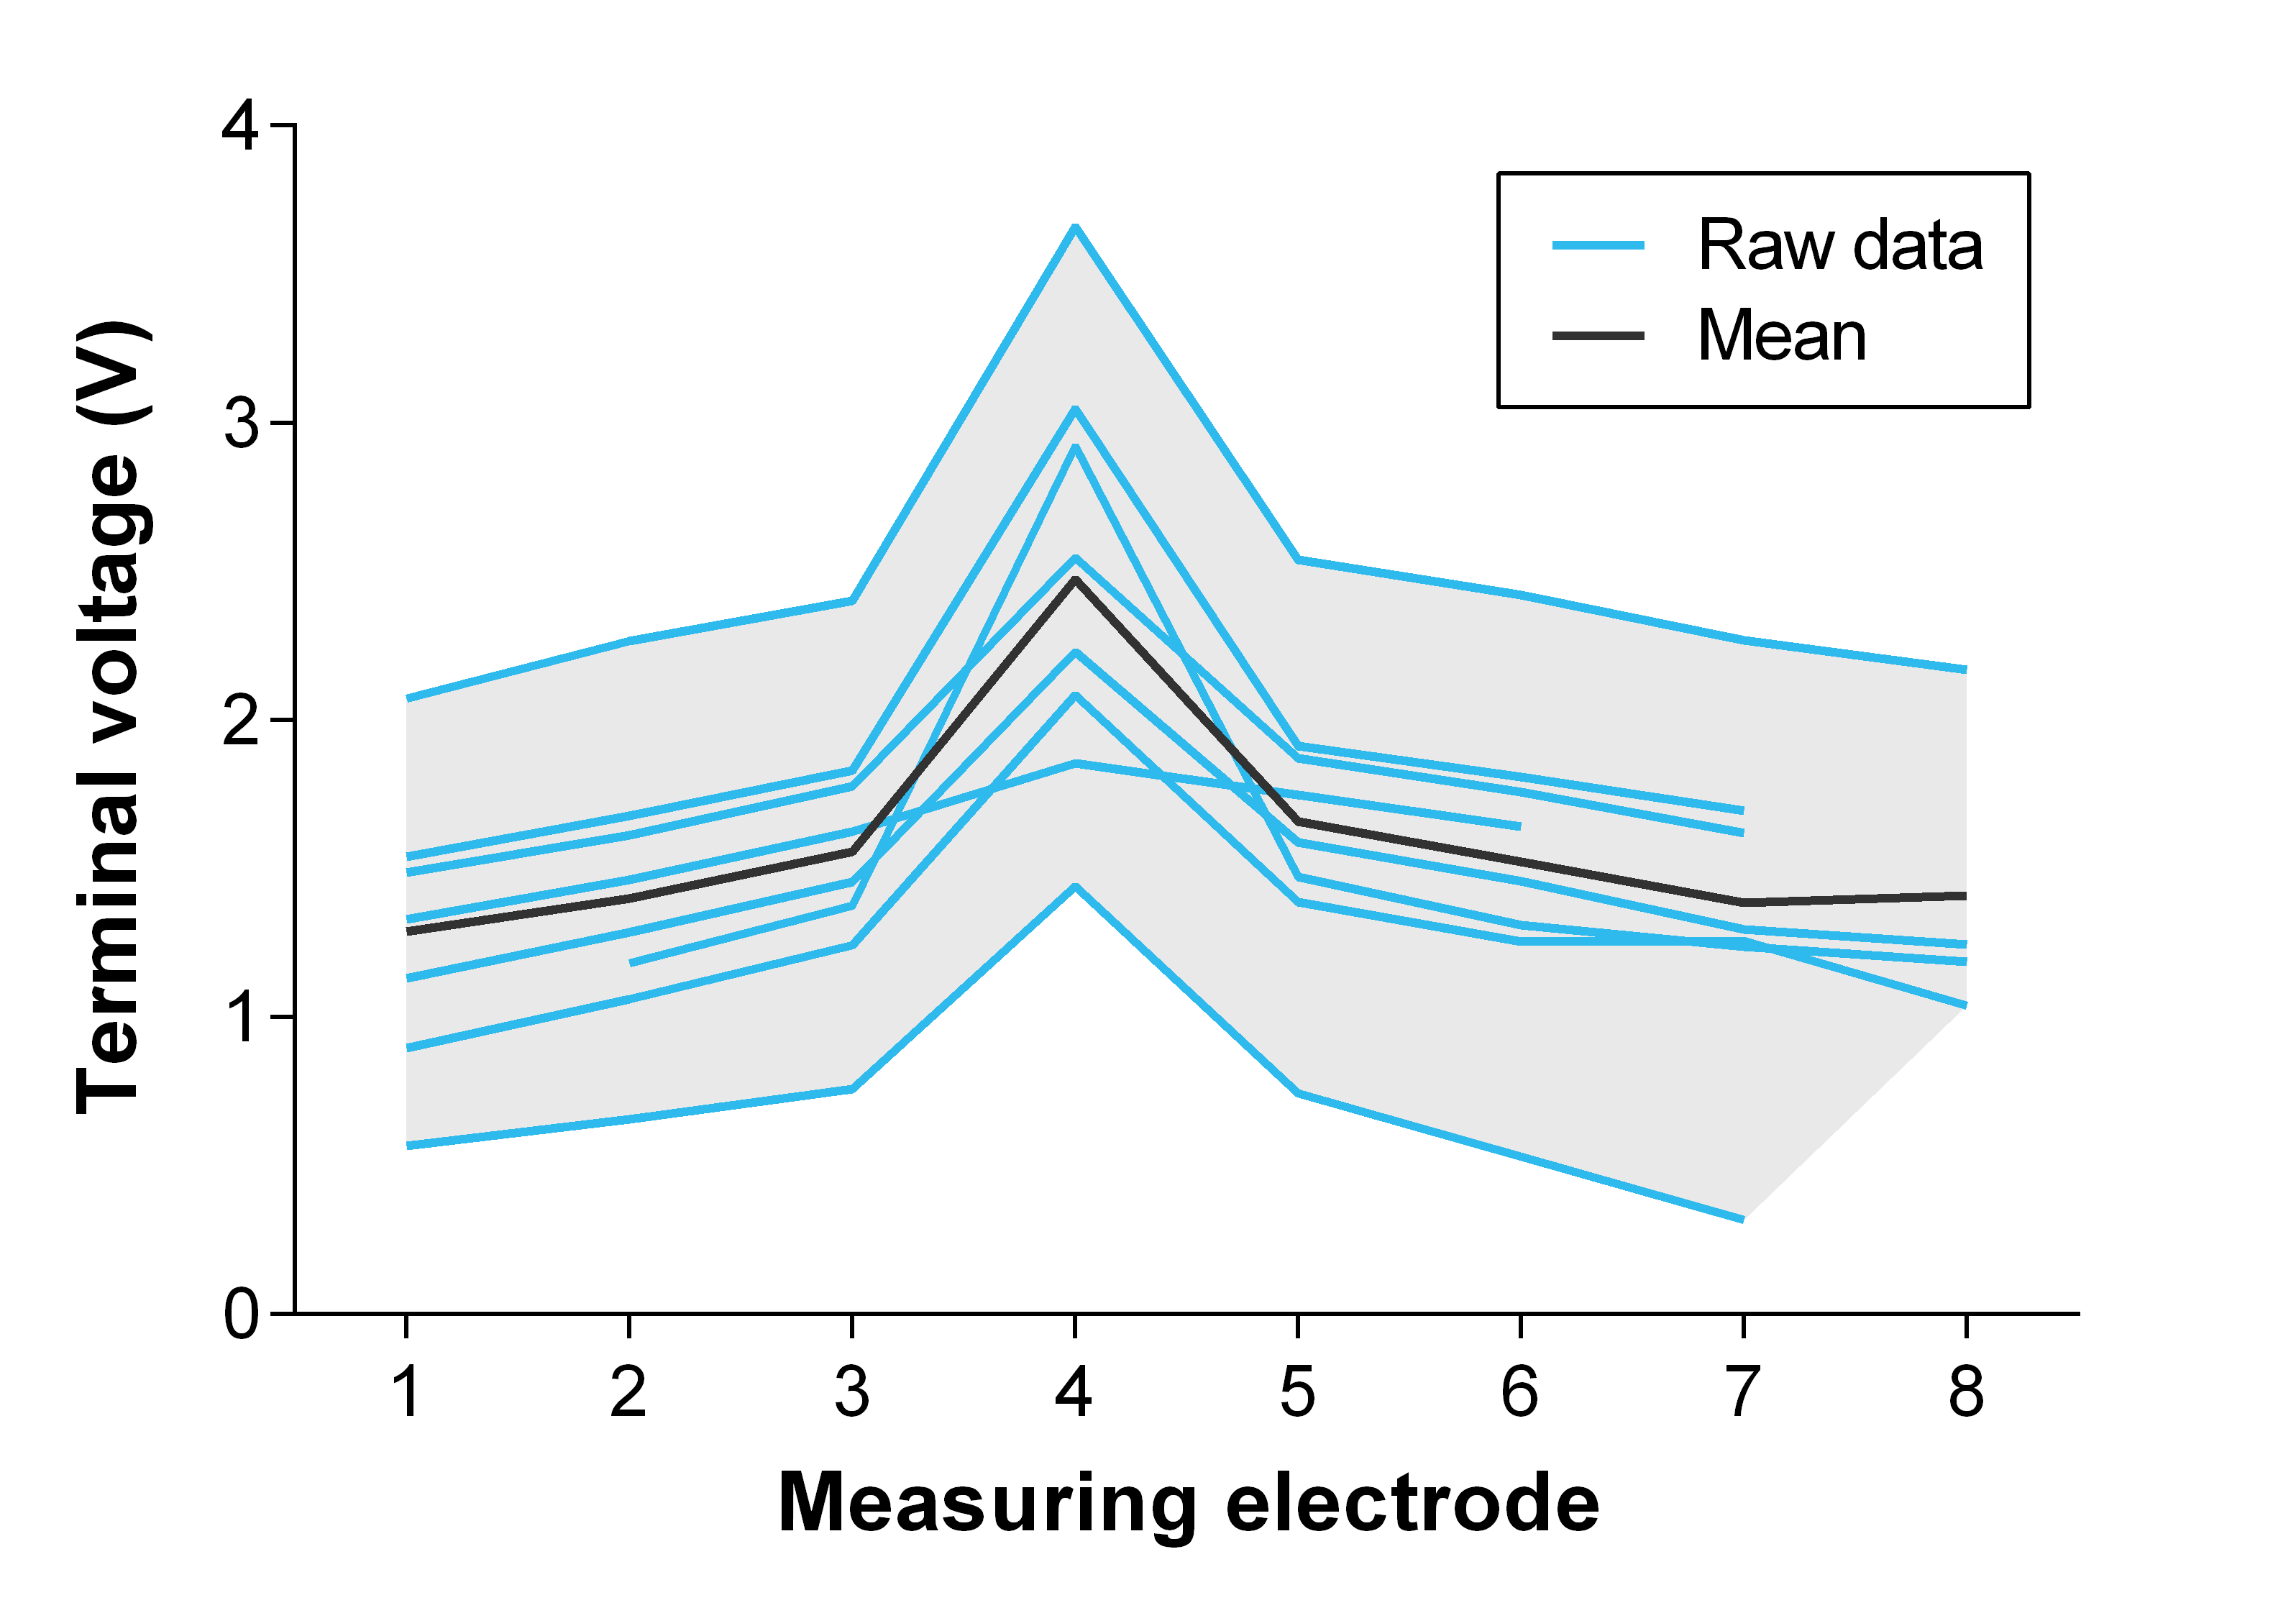
\includegraphics[height=7cm]{Validation/in_vivo_shefin}
	\caption[\textit{In vivo} voltage measurements along the array]{\textit{In
	vivo} voltage measurements (N=8) along the array during E4 stimulation.
	Shortened traces are likely due to tip fold-over or incomplete insertion. The
	shaded area represents the spread of \invivo{} results. (Copyright
	\textcopyright{} 2015, IEEE.)}
	\label{fig:in_vivo_data}
\end{figure}

The apical electrode (E8) was excluded from the comparisons because measurements
from that electrode could not be obtained in four of the eight guinea pigs. This
was likely due to the electrode tip folding over during insertion.

\begin{figure}[p]
	\centering
	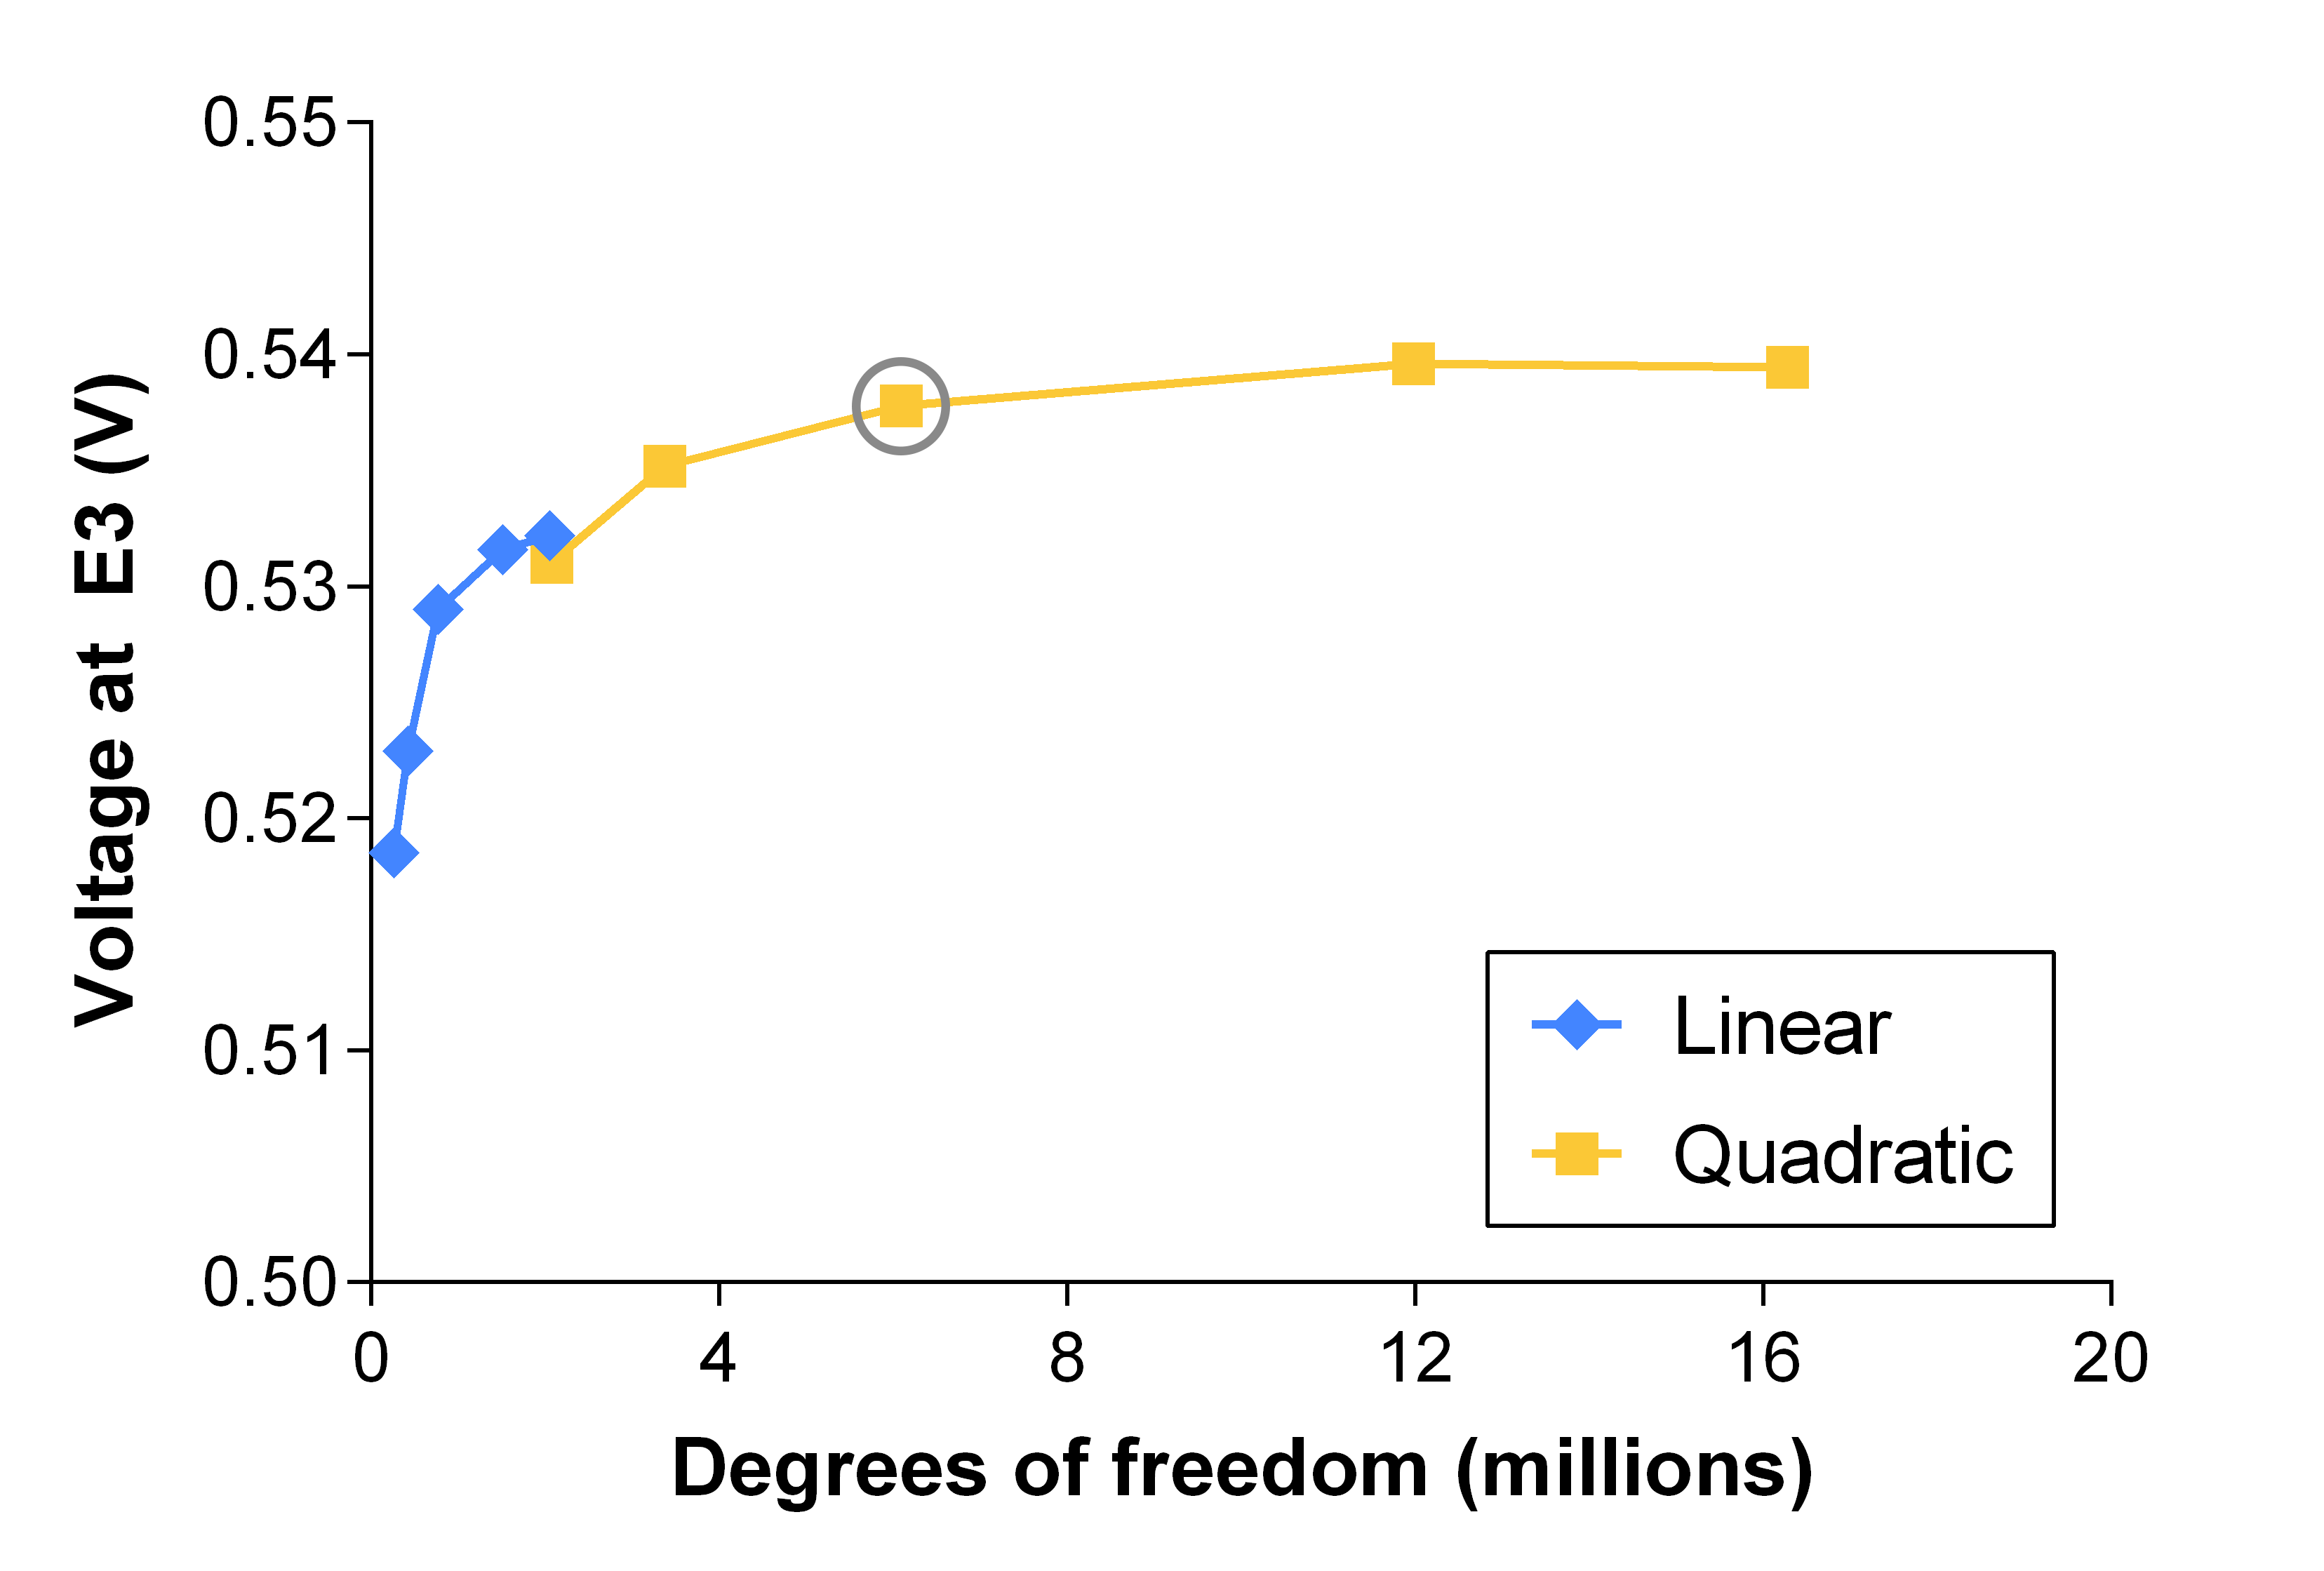
\includegraphics[height=7cm]{Validation/convergence_circled}
	\caption[Mesh convergence results]{Mesh convergence results for terminal voltage
	at E3 during stimulation at E4. The selected mesh exhibits only 0.3\% difference
	relative to the densest quadratic mesh (far right). (Copyright \textcopyright{}
	2015, IEEE.)}
	\label{fig:mesh_convergence}
\end{figure}

\subsection{Mesh Convergence}
\label{sect:mesh_convergence}

Each mesh was solved using both linear and quadratic elements. The coarsest
linear mesh had 262,620 degrees of freedom (DOFs) and the finest quadratic mesh
had 16,278,789 DOFs. Solution times ranged from 12 seconds to 2 hours per
simulation.

Figure~\ref{fig:mesh_convergence} indicates that the mesh with 6,092,537 DOFs is
well converged, with only 0.3\% difference relative to the densest quadratic
mesh that was tested. Solution time was about 30 minutes, striking a good
balance between accuracy and computational cost. All of the linearly discretised
meshes exhibited greater than 5\% difference. This suggests that linear shape
functions were not sufficient for capturing the electric field behavior in this
model (cf. Frijns~\etal~\cite{frijns1995}).

\subsection{Sensitivity of Terminal Voltage Predictions}

Table~\ref{table:voltage_sensitivity} shows the percentage impact of tissue
properties on terminal voltage predictions. These values were calculated
relative to the base case and classified as either negligible (less than 1\%
difference), weak (1--5\%), or strong (more than 5\%), again based on the 5\%
sufficiency criteria of Frijns~\etal~\cite{frijns1995}. For this model, the
resistivities of most tissues had either a negligible or weak effect on terminal
voltages. The exceptions were bone, perilymph, and nerve. Temporal bone
resistivity was the most sensitive, with differences of up to 90.8\% relative to
the base case. At extreme literature values for otic capsule
resistivity~\cite{haueisen1997,williams1996}, up to 59\% difference was
observed. Treating bone with a homogeneous resistivity of 6.41~$ \Omega \cdot$m
underestimated terminal voltages relative to the base case (see
Figure~\ref{fig:voltage_sensitivity_TR}). Perilymph had a particularly strong
effect at the stimulating electrode and was notably the only tissue to change
the shape of the profile. Nerve resistivity had up to 5.79\% impact on terminal
voltages.

\begin{table}
	\mathversion{sans}
	\centering
	\sffamily
	\small
	\caption[Sensitivity of terminal voltages to tissue resistivities]{Sensitivity
	of terminal voltages to tissue resistivities. Deltas were calculated relative
	to the base case. Weak (+) and strong (++) impact tissues are indicated.
		{\textsuperscript{a}}Resistivity changed from base value by a factor of two.
		{\textsuperscript{b}}Upper and lower resistivity limits based on extreme
		values from literature, as indicated.
		{\textsuperscript{c}}Resistivity changed from base value by a factor of ten.
	}
	\label{table:voltage_sensitivity}
	
	\begin{tabularx}{0.85\textwidth}{X c c c}
		\toprule
		\textbf{Tissue}	& \multicolumn{2}{c}{\textbf{Deviation from base case (\%)}}
			& \textbf{Impact} \\
						& \textbf{~~~~~~~Mean~~~~~~~} & \textbf{Max}
			& \\
		\midrule
		
		\csvreader[late after line=\\]%
			{Validation/voltage_sensitivity.csv}%
			{1=\tissue,2=\mean,3=\max,4=\strength}%
 			{\tissue & \mean & \max & \strength}%
		\bottomrule
	\end{tabularx}
	
\end{table}

\begin{figure}
	\centering
	
	\begin{subfigure}[t]{\textwidth}
        \centering
        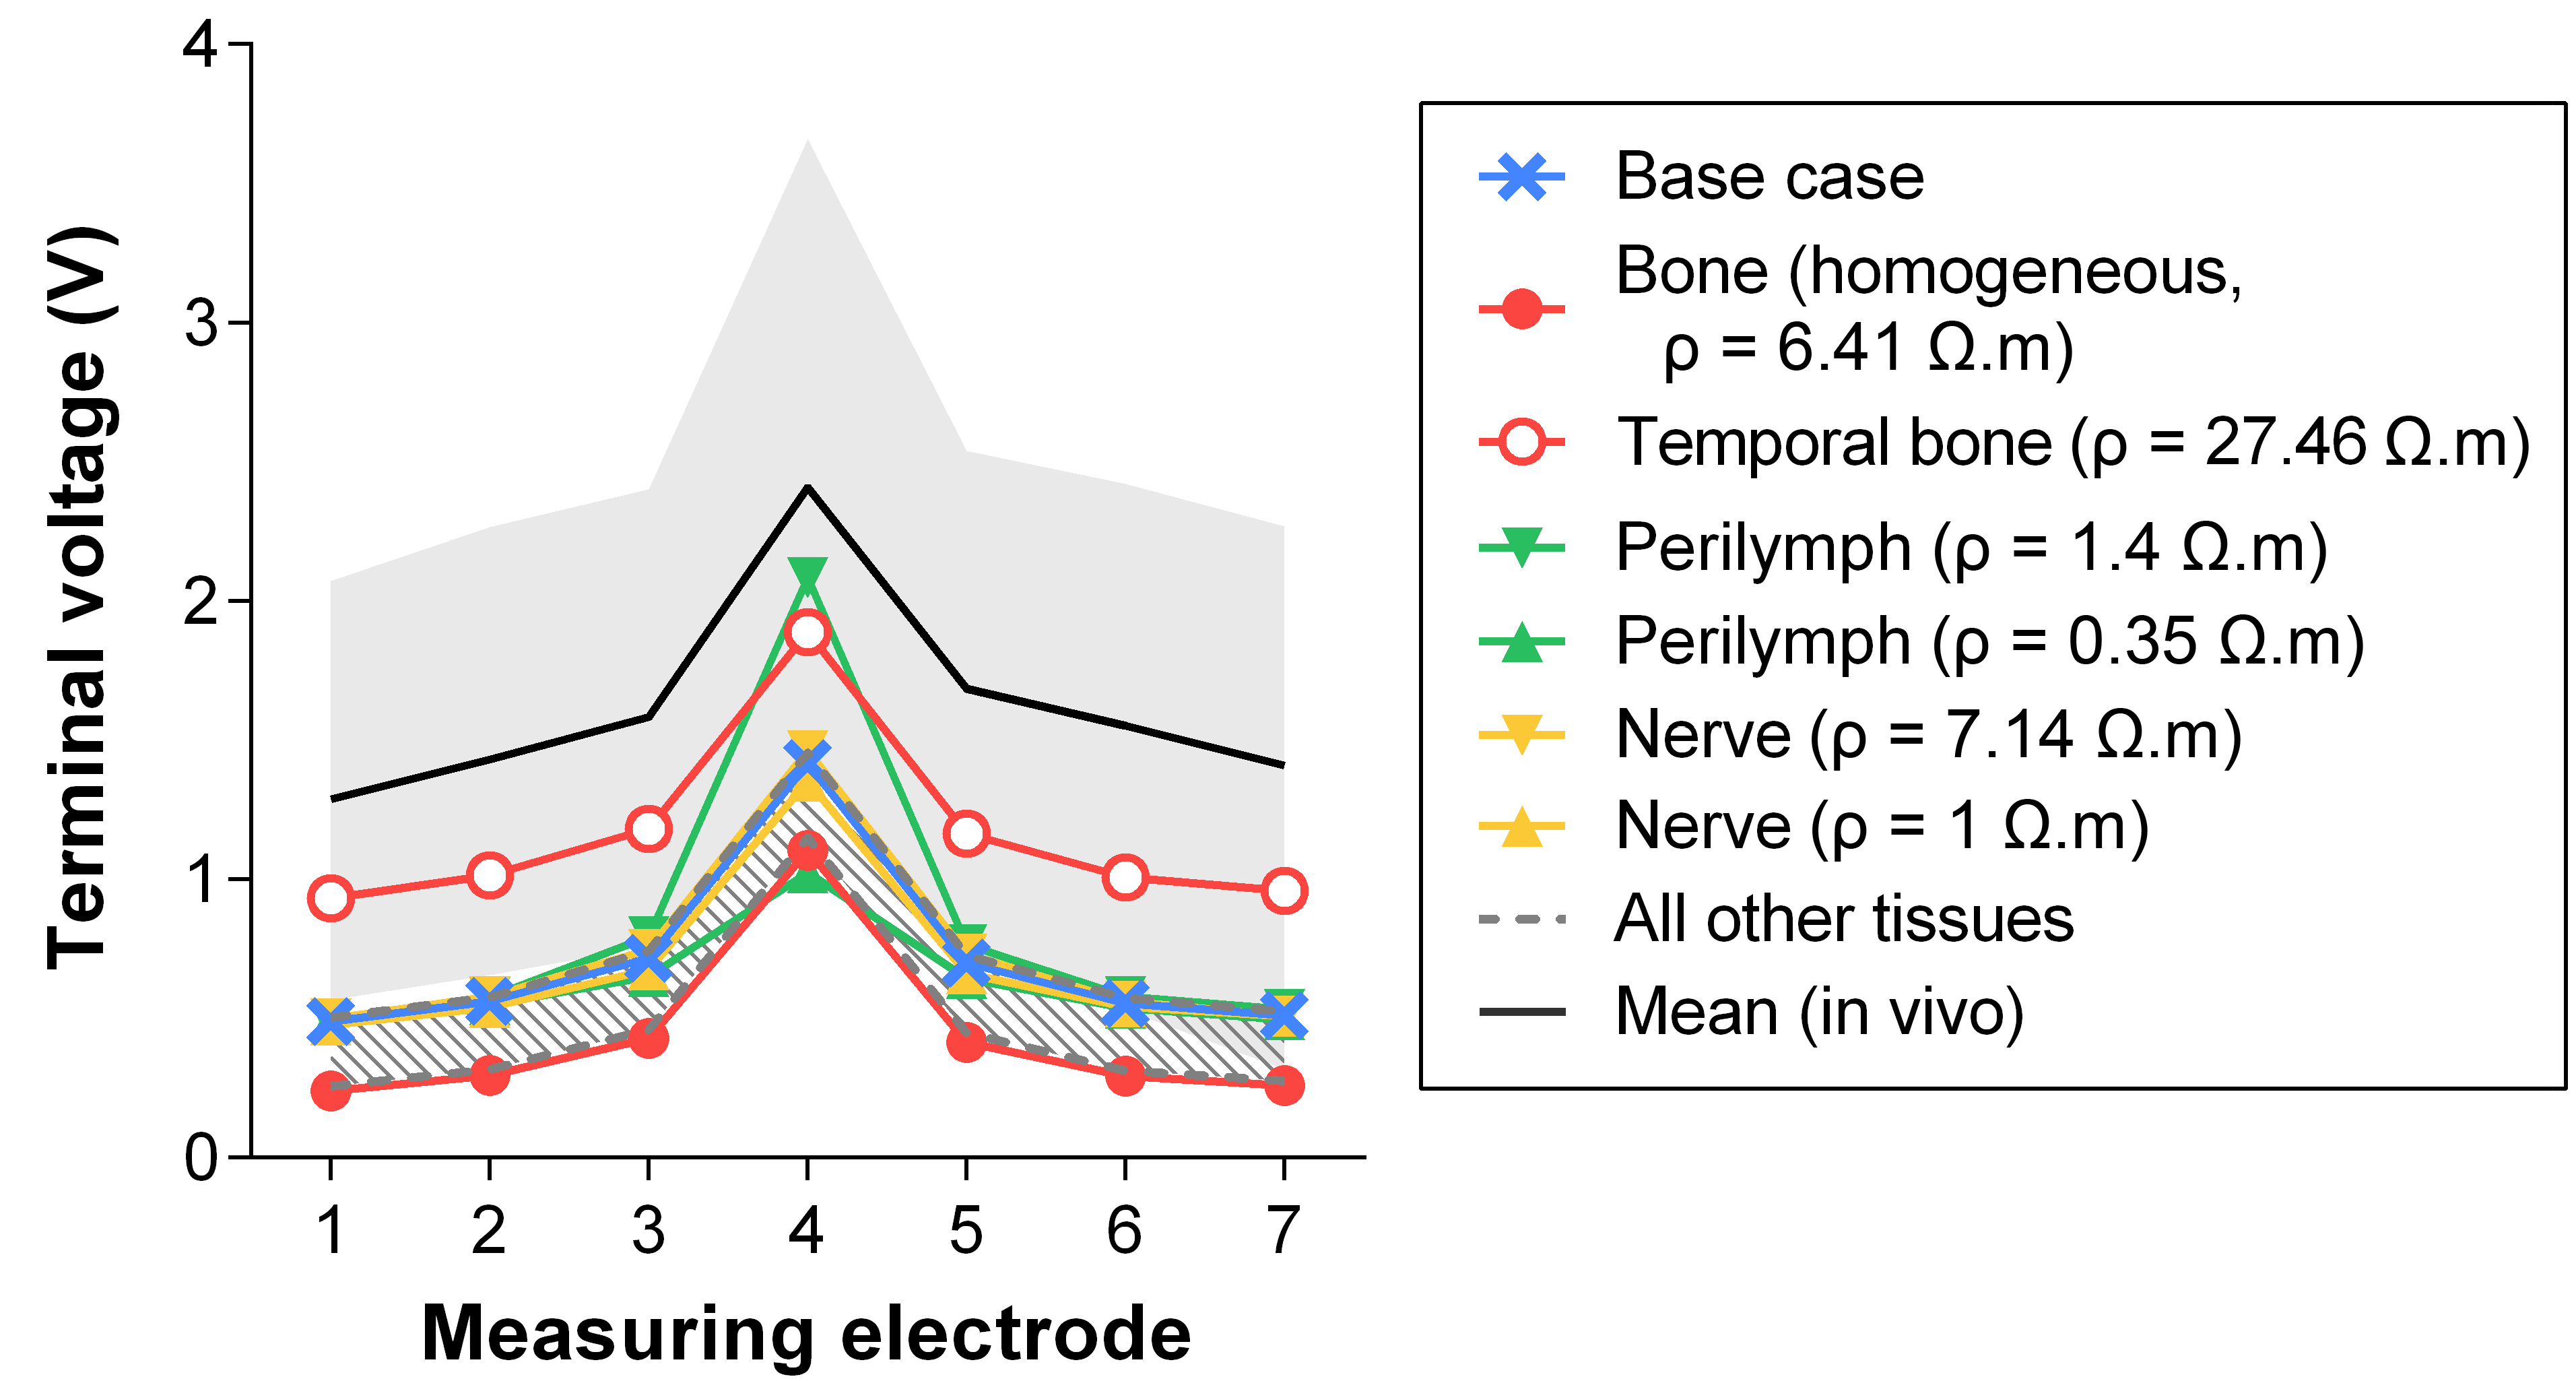
\includegraphics[height=6.4cm]{Validation/voltage_sensitivity_TR}
        \caption{Sensitivity to tissue resistivities}
        \label{fig:voltage_sensitivity_TR}
    \end{subfigure}\\%
    \vspace{1em}%
    \begin{subfigure}[t]{\textwidth}
        \centering
        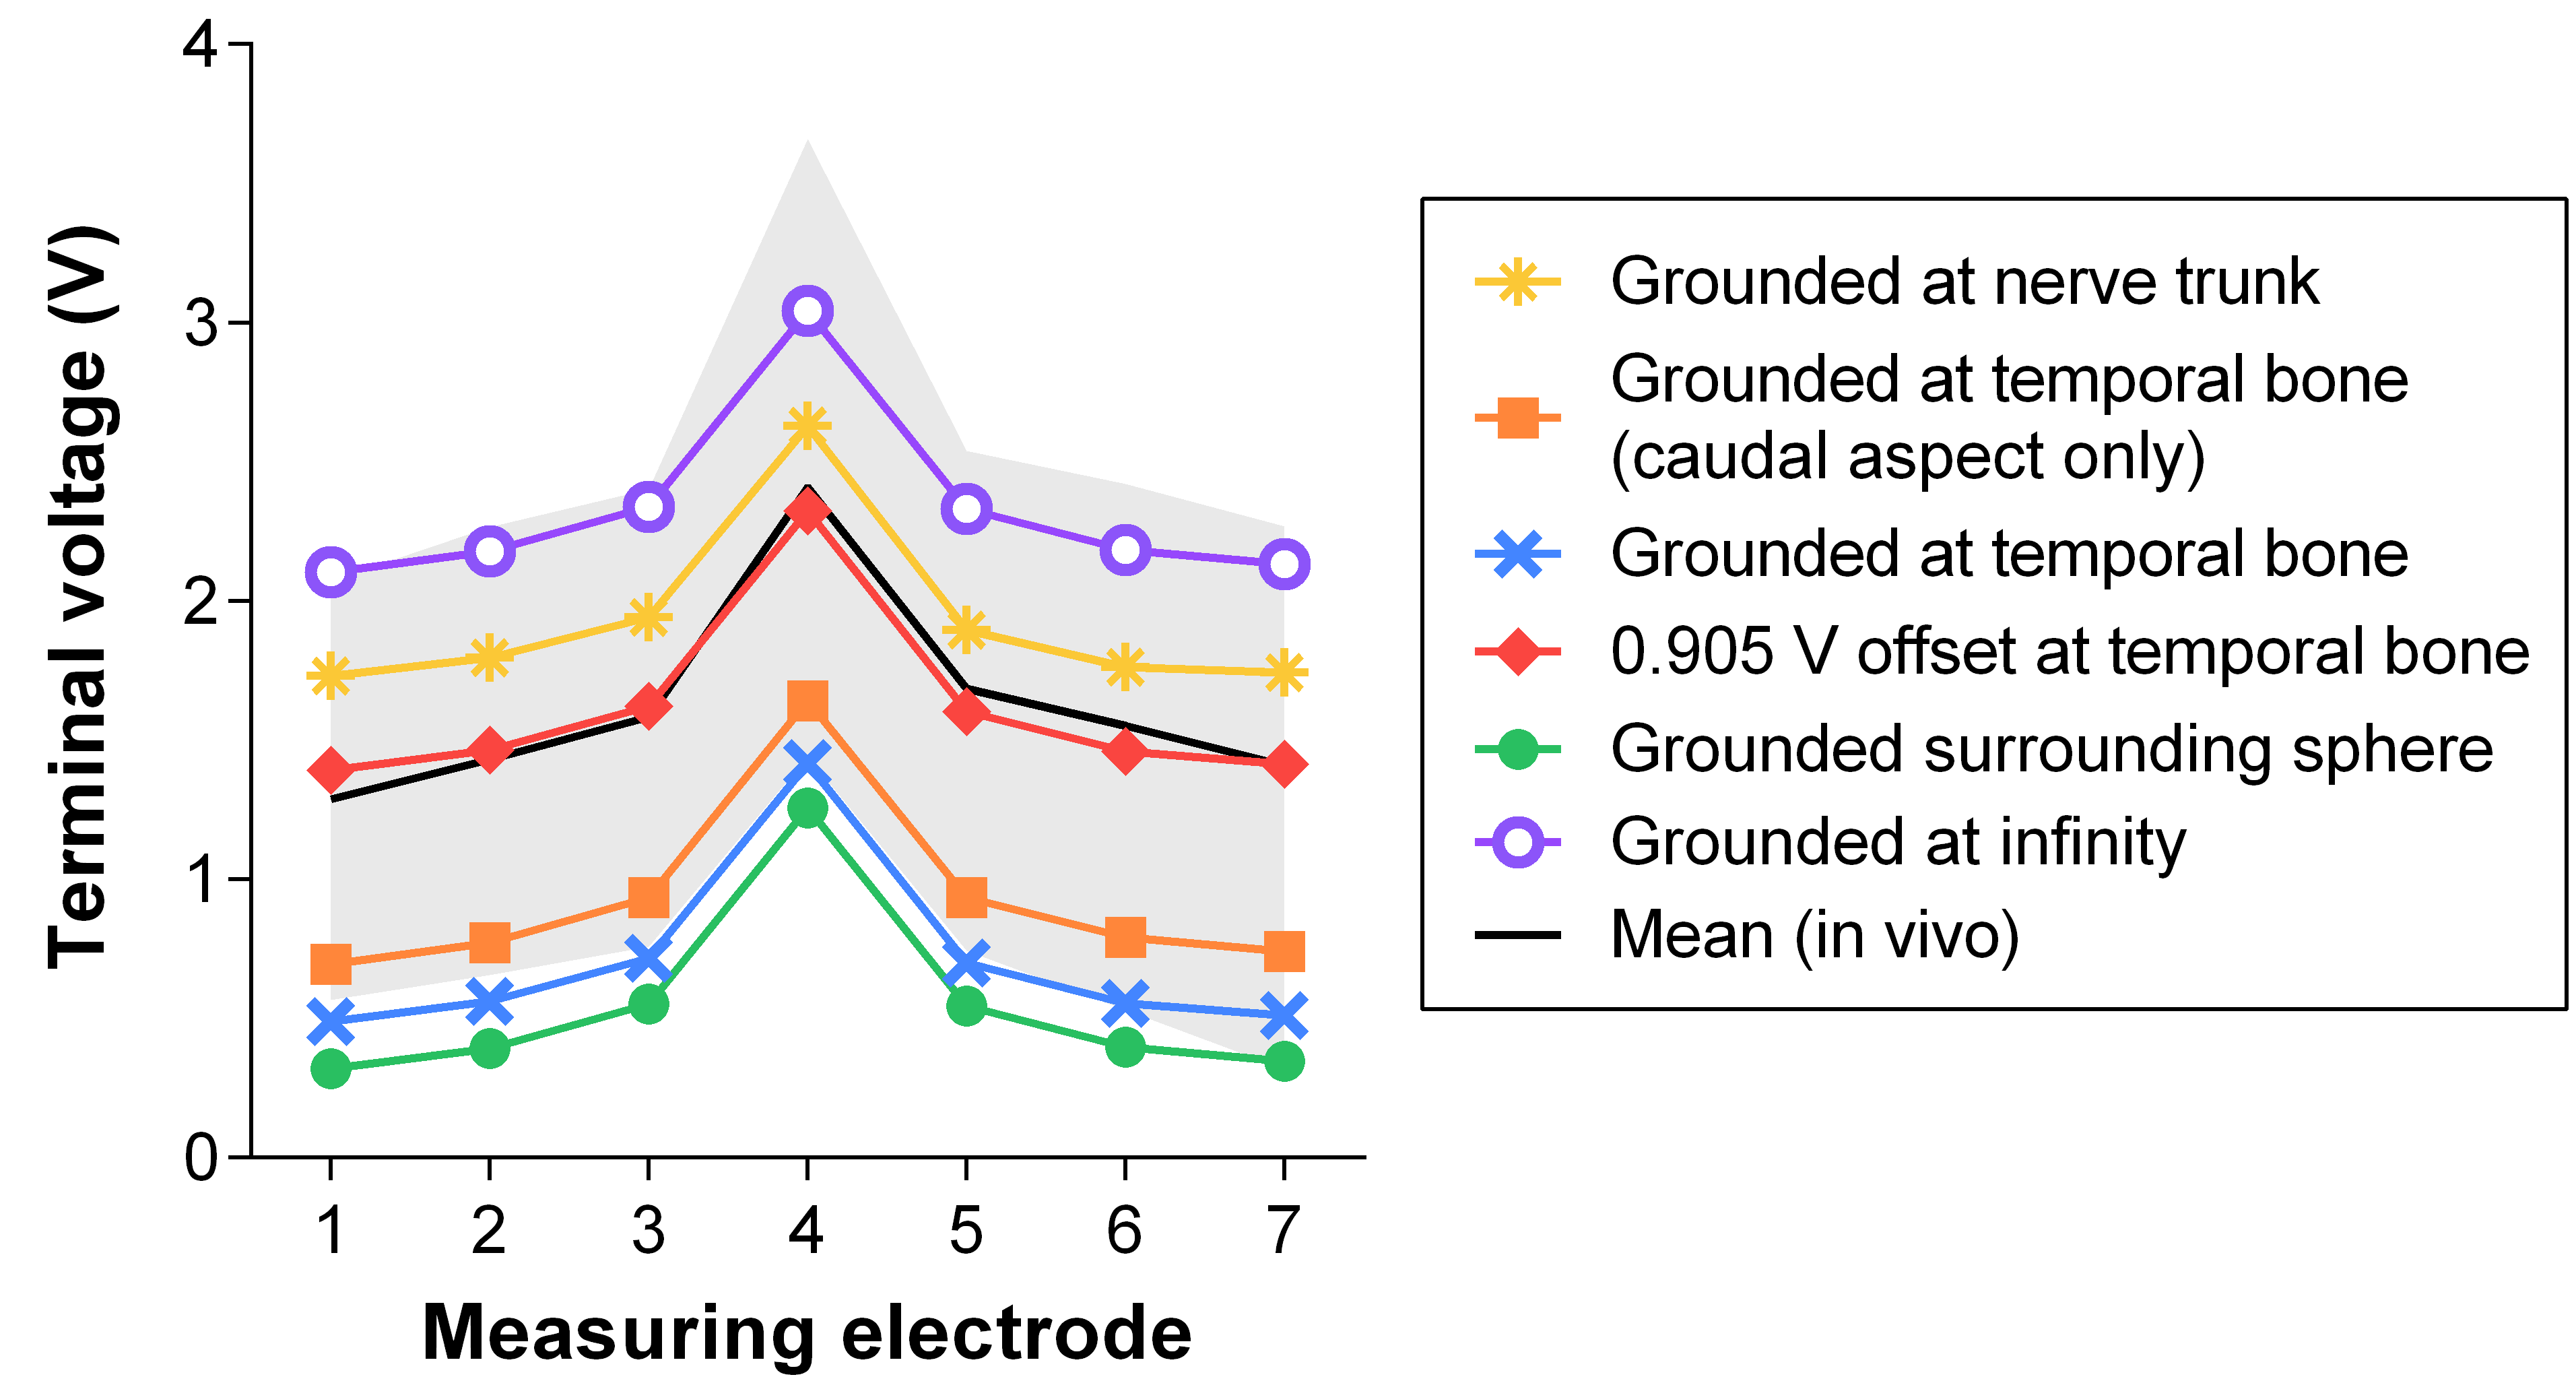
\includegraphics[height=6.4cm]{Validation/voltage_sensitivity_BC}
        \caption{Sensitivity to boundary conditions}
        \label{fig:voltage_sensitivity_BC}
    \end{subfigure}%
    
    \caption[Sensitivity of terminal voltages]{Sensitivity of terminal voltages
    to key model inputs. Base case values are marked with blue crosses.
    The light grey areas represent the range of \invivo{} voltage measurements
    from Figure~\ref{fig:in_vivo_data}. (a) Most tissues had little impact on
    the \insilico{} predictions, and almost all data points fell outside the
    \invivo{} range. (b) Boundary conditions had virtually no effect on the
    shape of the profile, but strongly affected the voltage magnitudes. (Copyright
	\textcopyright{} 2015, IEEE.)}
	\label{fig:voltage_sensitivity}
\end{figure}

Figure~\ref{fig:voltage_sensitivity_BC} compares the \insilico{} and \invivo{}
terminal voltages for each of the tested boundary conditions. The shape of the
profile was unaffected, but a wide spread of voltage magnitudes was observed.
Grounding at infinity or at the nerve trunk overestimated voltages along the
array, relative to the observed \invivo{} mean. In contrast, grounding the
surrounding sphere or part thereof led to substantial underestimates, with
smaller grounding areas corresponding to higher terminal voltages. Some of these
fell outside the range of observed \invivo{} measurements.

\begin{figure}
	\centering
	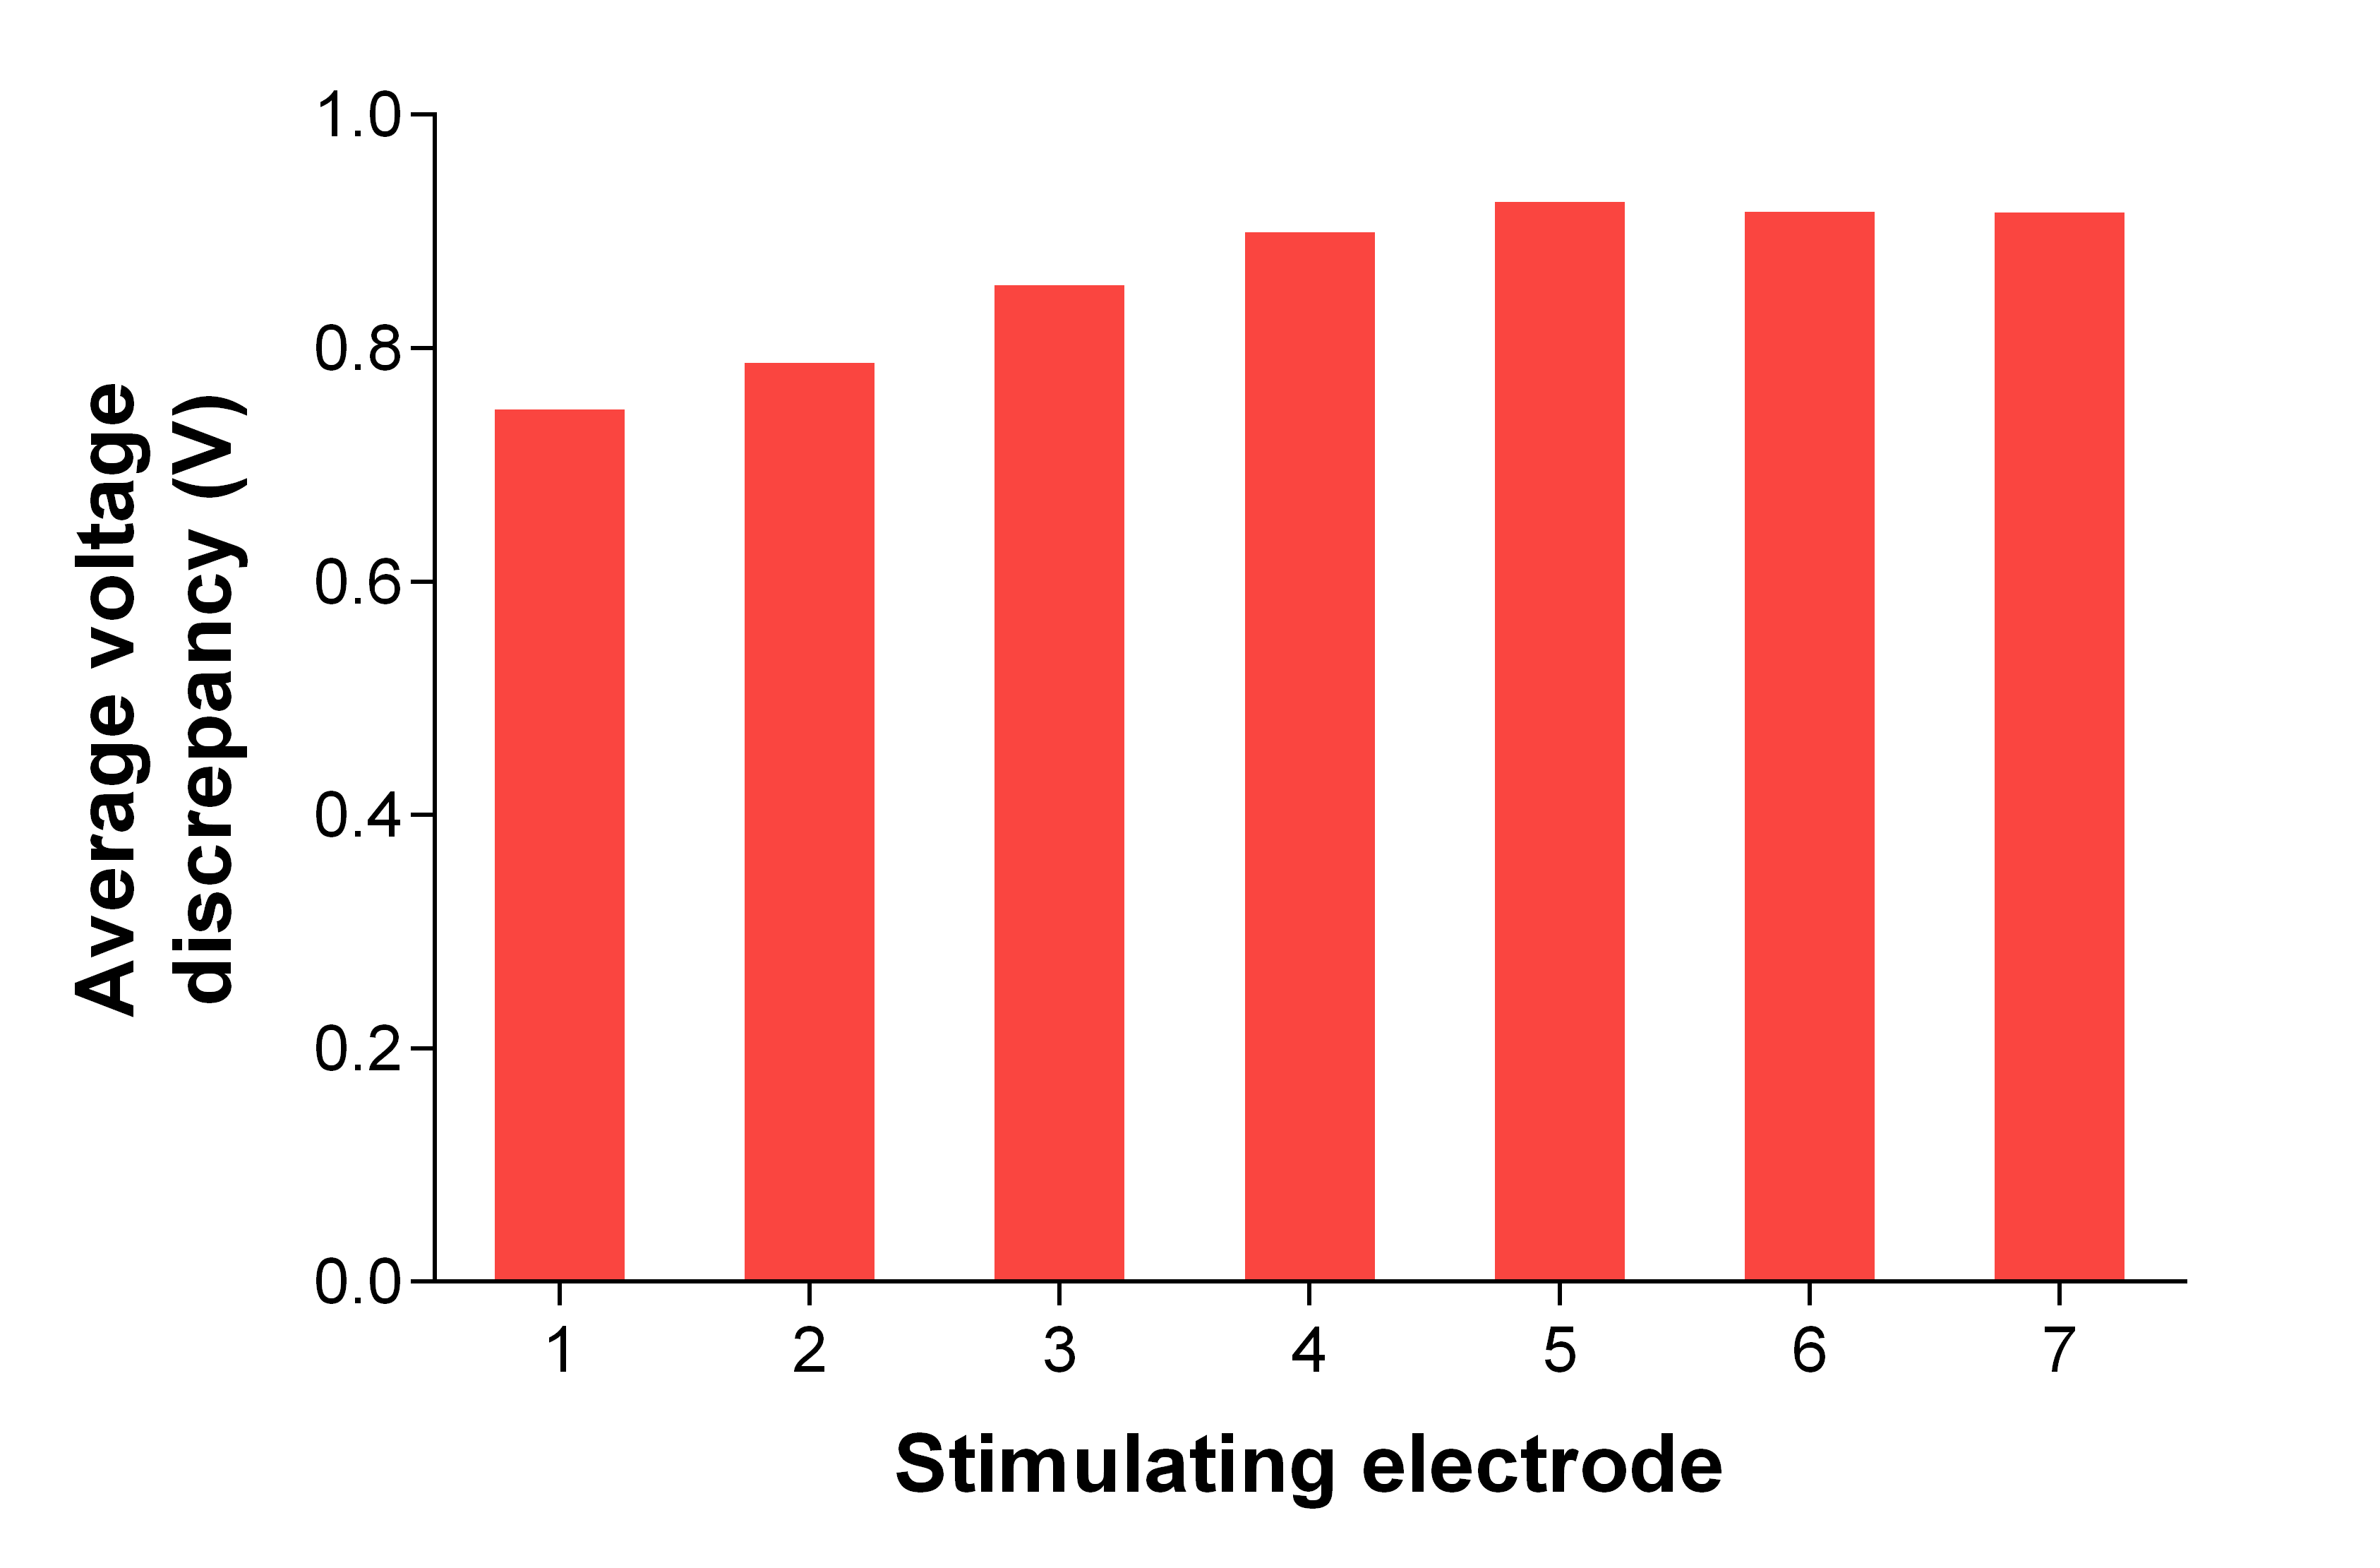
\includegraphics[height=7cm]{Validation/offsets}
	\caption[Voltage offset required to
	match the mean \invivo{} results]{Voltage offset required to
	match the mean \invivo{} results changed with the location of current
	injection. Offset values were lower for basal electrodes, and levelled off
	between E4 and E7. (Copyright \textcopyright{} 2015, IEEE.)}
	\label{fig:offsets}
\end{figure}

Offset values required to match the \invivo{} average were found to vary with
the location of current injection, as shown in Figure~\ref{fig:offsets}. For
stimulation at E4, a 0.905~V offset on the temporal bone surface was required to
match the \invivo{} measurements, equivalent to a 905~$ \Omega $ of resistance
to ground. This compares well with values in the literature. Von \bekesy{}
estimated the resistance between the round window and the body at 2000~$ \Omega
$~\cite{vonbekesy1960}, and Johnstone~\etal{} estimated total resistance to the
monopolar return to be 1580~$ \Omega $~\cite{johnstone1966}. Both of these are
slightly higher than the \insilico{} offset voltages obtained here, but this is
expected since they were measured from inside the cochlea and so include
additional resistance from the cochlear tissues and some surrounding bone.

\subsection{Effect on Current Pathways}

Streamline plots revealed that current spread in the near-field was relatively
insensitive to both tissue properties and boundary conditions, leading to
similar gradients of voltage falloff as shown in
Figure~\ref{fig:voltage_sensitivity}. Beyond the scala tympani however, current
flow patterns were noticeably different. Figure~\ref{fig:valid_streamlines}
shows that current paths were strongly dependent on the prescribed boundary
condition. Grounding the nerve (Figure~\ref{fig:valid_streams_nerve}) was the
most distinct, with streamlines reconverging at the grounded nerve surface and
an obvious edge effect around its periphery.  Grounding the entire surrounding
sphere (Figure~\ref{fig:valid_streams_sph}) resulted in omnidirectional current
spread beyond the cochlea, as did grounding at infinity
(Figure~\ref{fig:valid_streams_inf}). Restricting the grounding surface to a
quadrant (Figure~\ref{fig:valid_streams_caudal}) or hemisphere
(Figure~\ref{fig:valid_streams_hemi}) imposed a sense of directionality on the
exit pathway. Lastly, applying a voltage offset on the temporal bone surface
produced virtually identical streamlines as grounding it.

\begin{figure}
	\centering
	
	\begin{subfigure}[t]{0.32\textwidth}
        \centering
        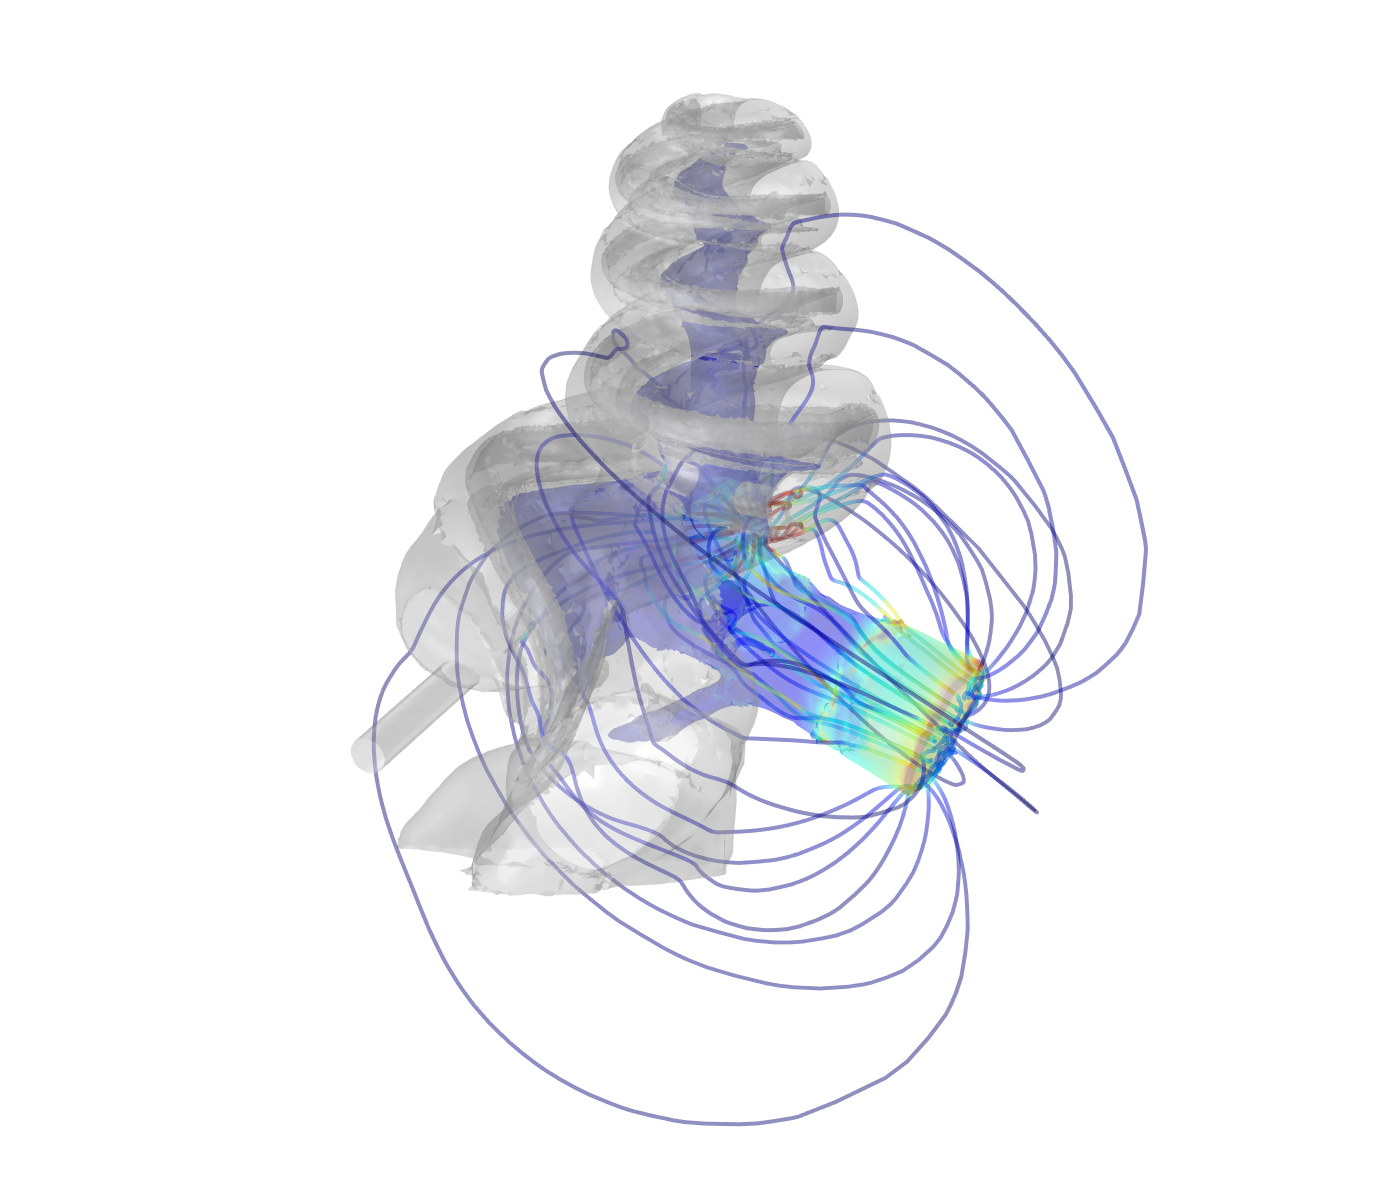
\includegraphics[height=4.5cm,trim={12mm 0 0 0},clip]
        	{Validation/streamlines-term4-nrvD_gnd-bare}
        \captionsetup{margin={-0.2cm,0cm}}
        \caption{}
        \label{fig:valid_streams_nerve}
    \end{subfigure}%
	\begin{subfigure}[t]{0.34\textwidth}
        \centering
        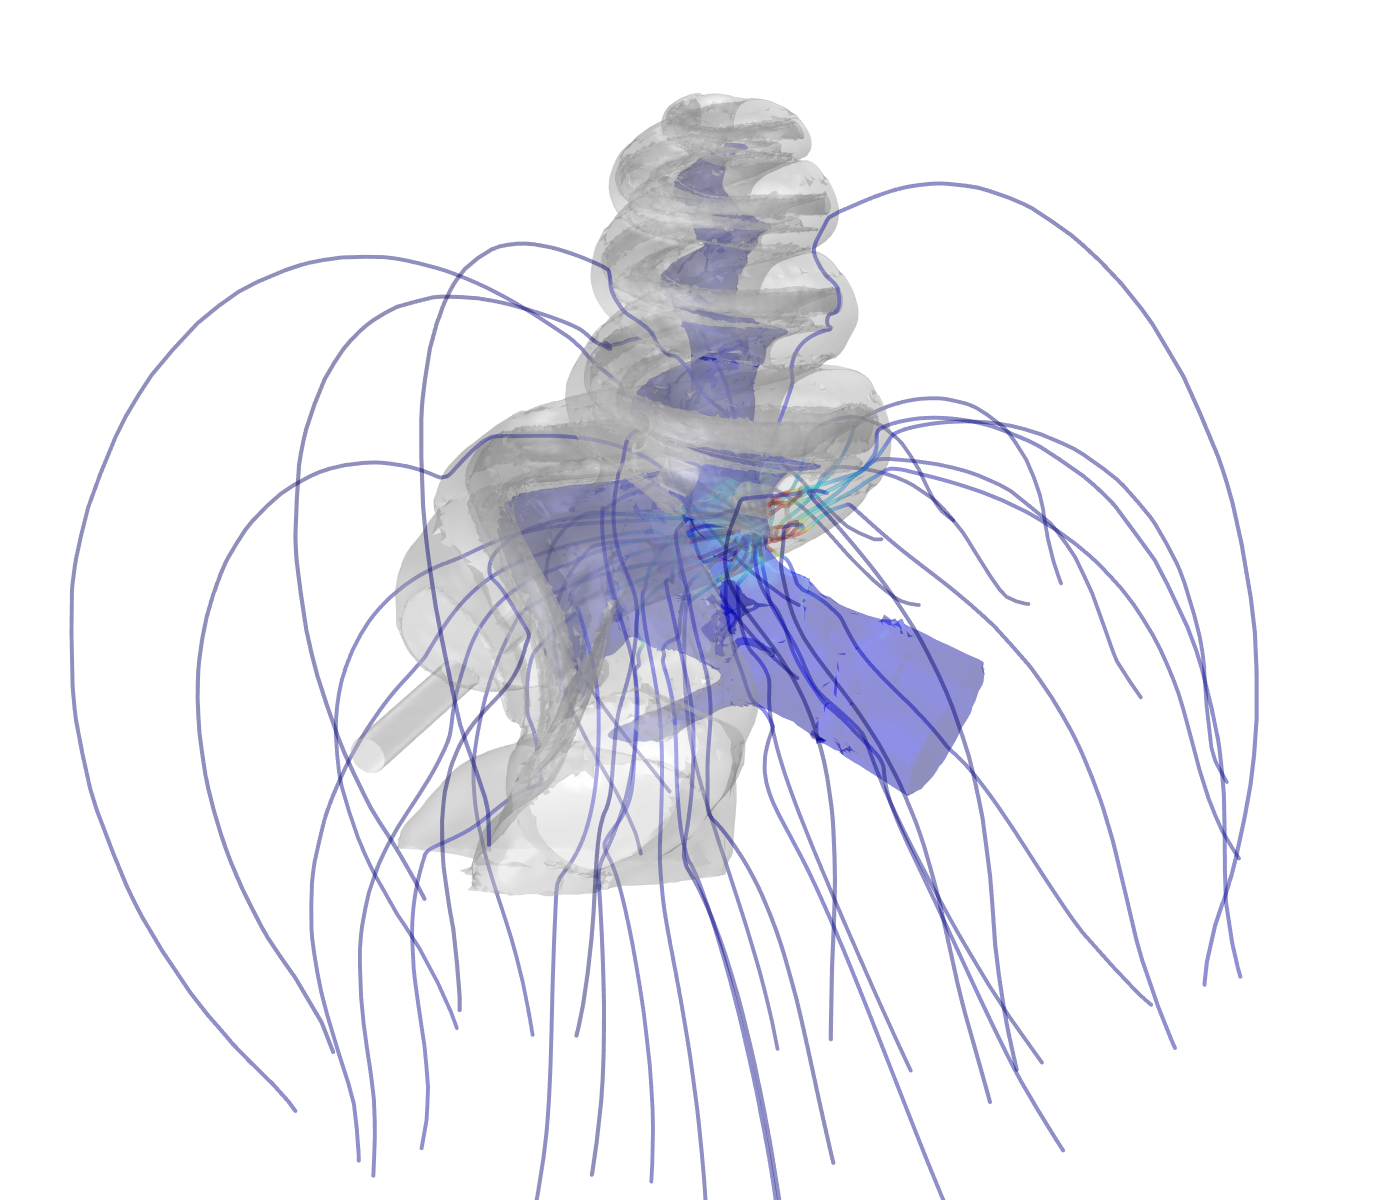
\includegraphics[height=4.5cm]{Validation/streamlines-term4-caud_gnd-bare}
        \caption{}
        \label{fig:valid_streams_caudal}
    \end{subfigure}%
	\begin{subfigure}[t]{0.34\textwidth}
        \centering
        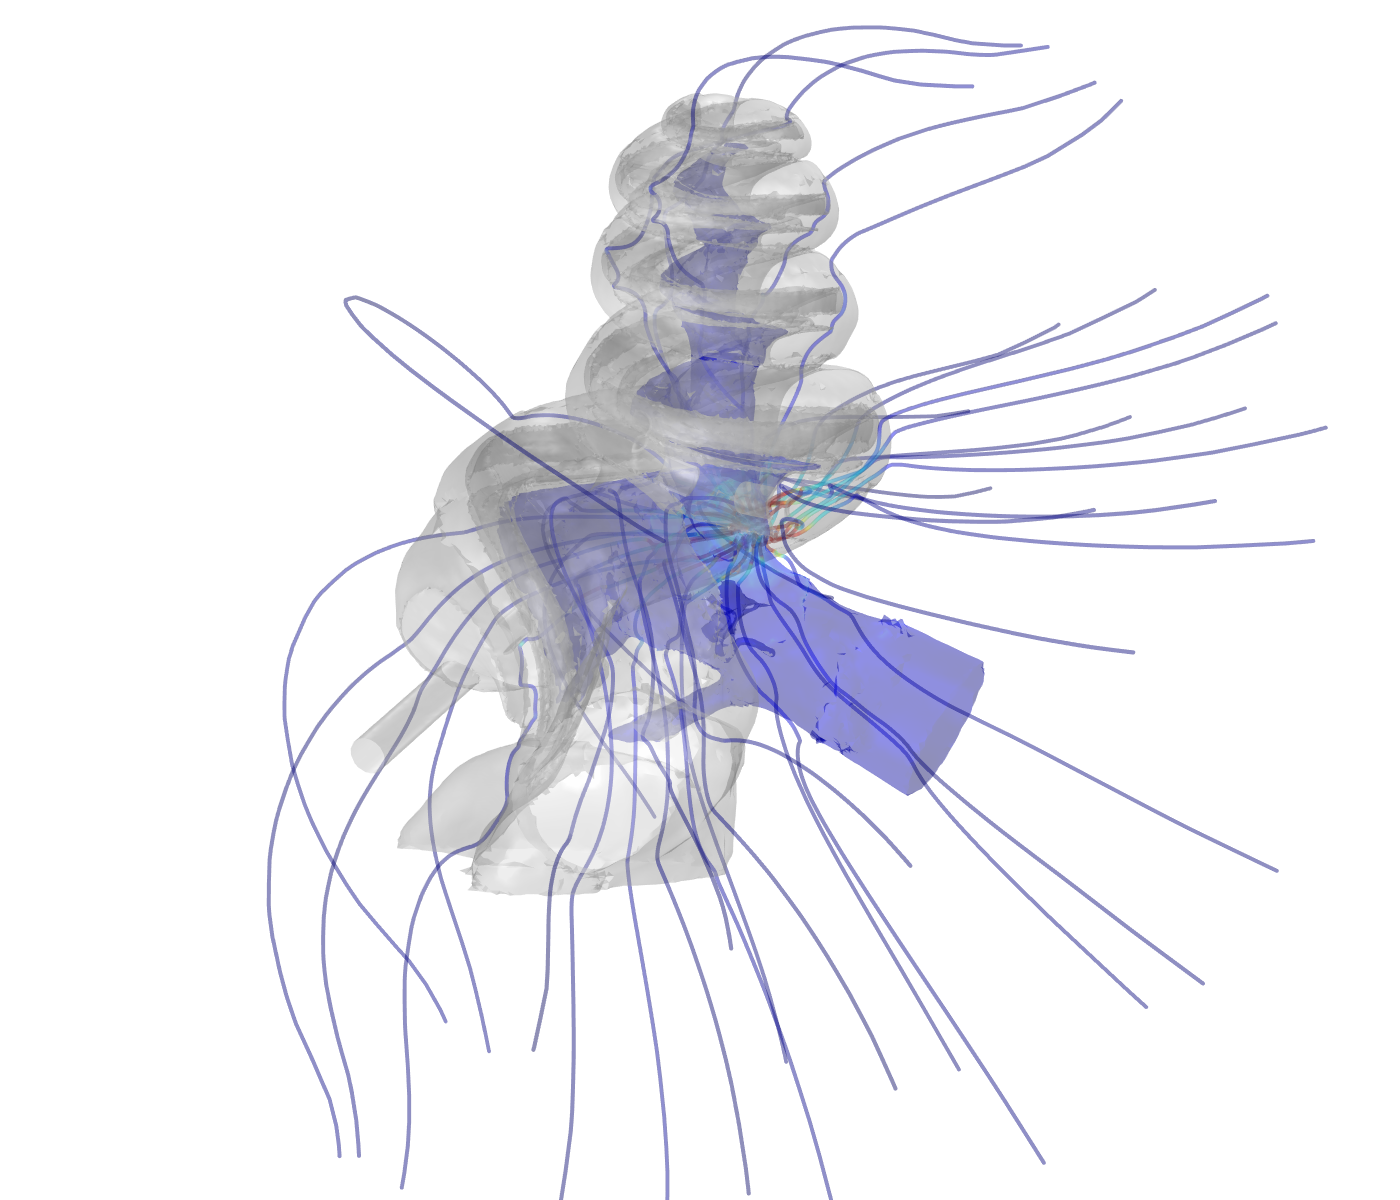
\includegraphics[height=4.5cm]{Validation/streamlines-term4-hemi_gnd-bare}
        \caption{}
        \label{fig:valid_streams_hemi}
    \end{subfigure}\\%
    \vspace{0.5em}\hspace{1cm}%
    \begin{subfigure}[t]{0.34\textwidth}
        \centering
        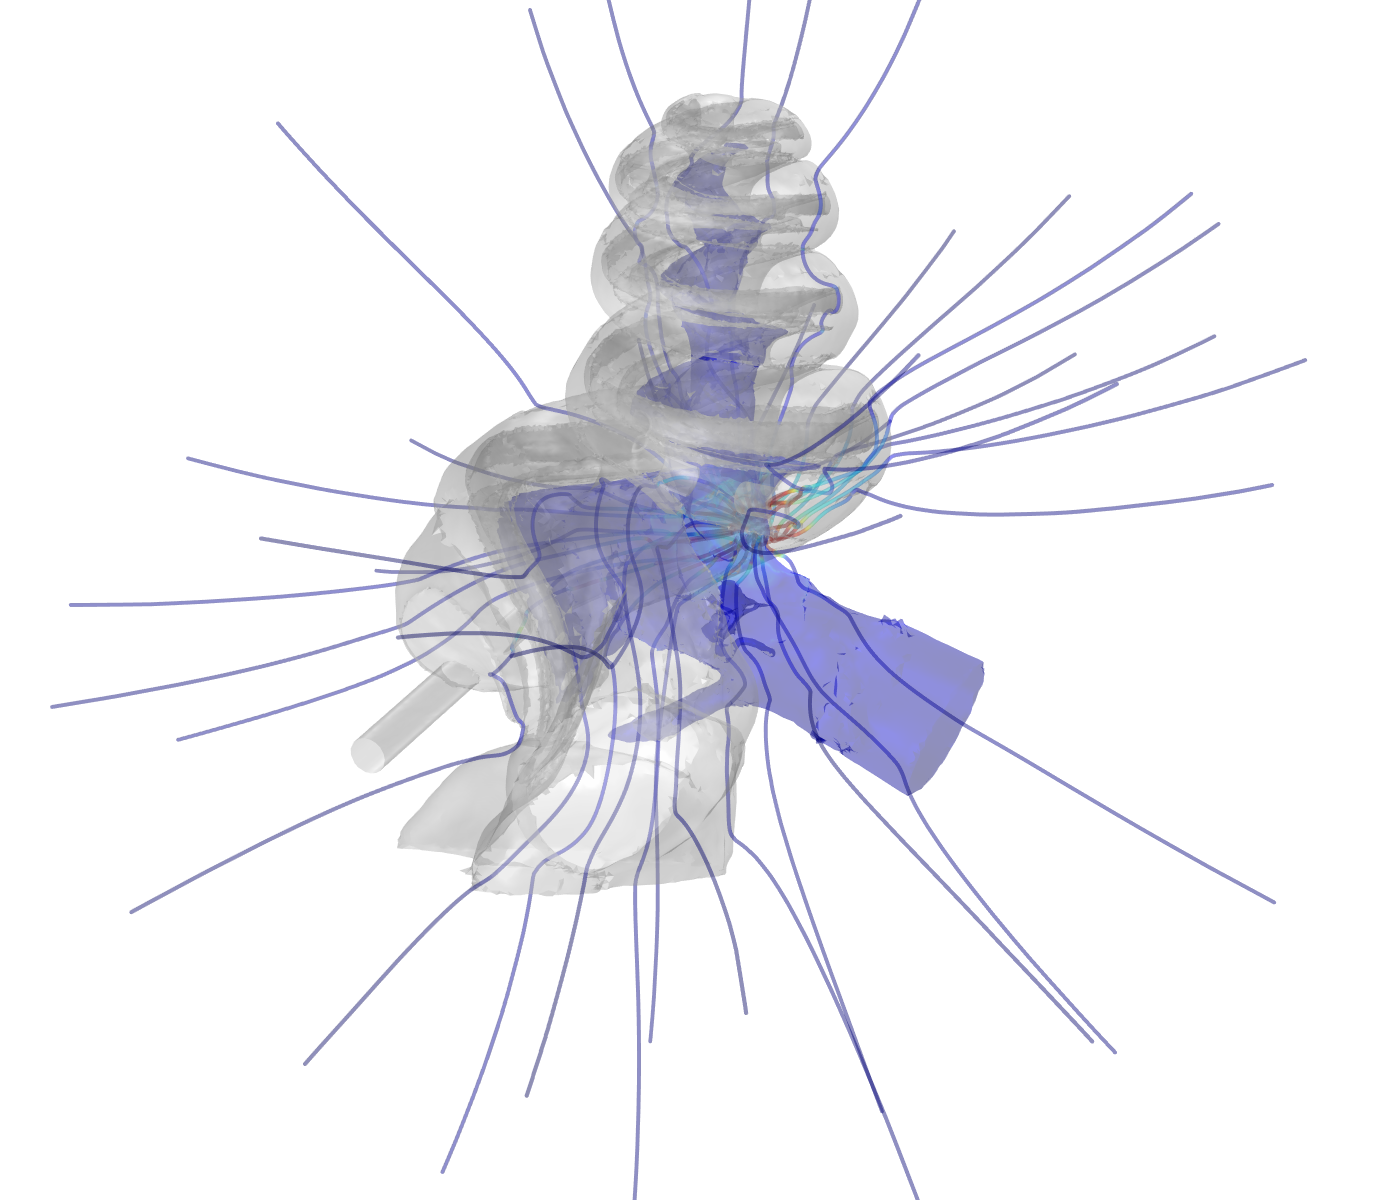
\includegraphics[height=4.5cm]{Validation/streamlines-term4-sph_gnd-bare}
        \caption{}
        \label{fig:valid_streams_sph}
    \end{subfigure}%
    \begin{subfigure}[t]{0.34\textwidth}
        \centering
        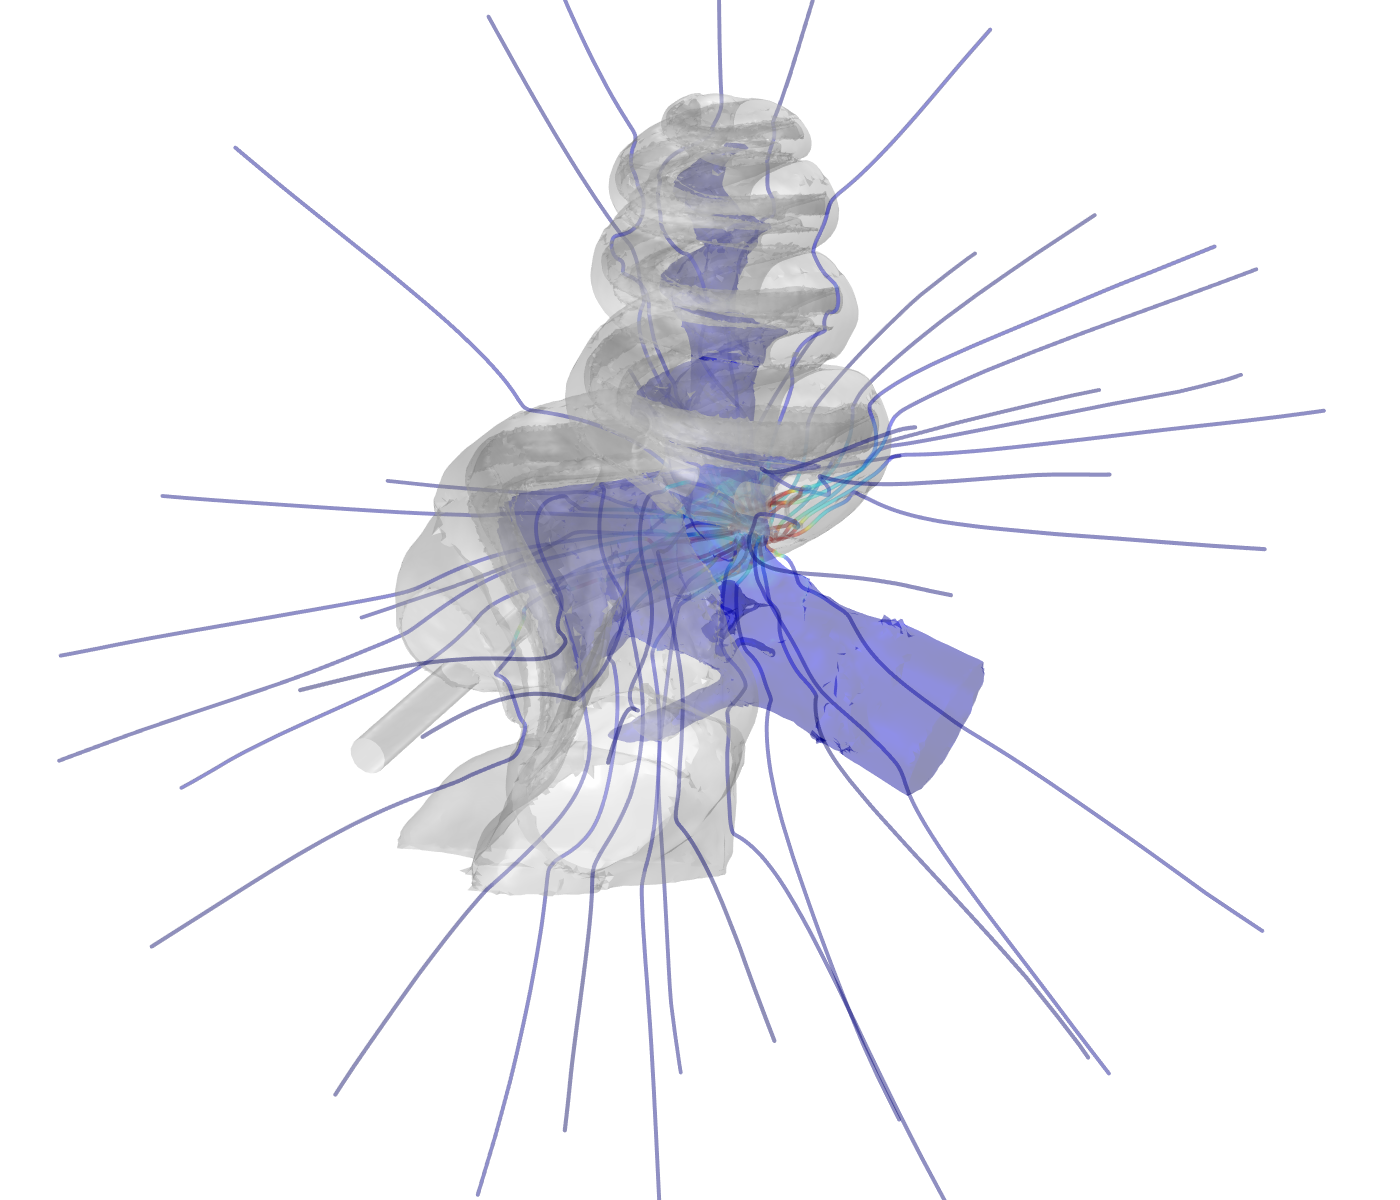
\includegraphics[height=4.5cm]{Validation/streamlines-term4-inf_gnd-bare}
        \caption{}
        \label{fig:valid_streams_inf}
    \end{subfigure}%
    ~~%
    \begin{subfigure}[t]{0.09\textwidth}
        \centering
        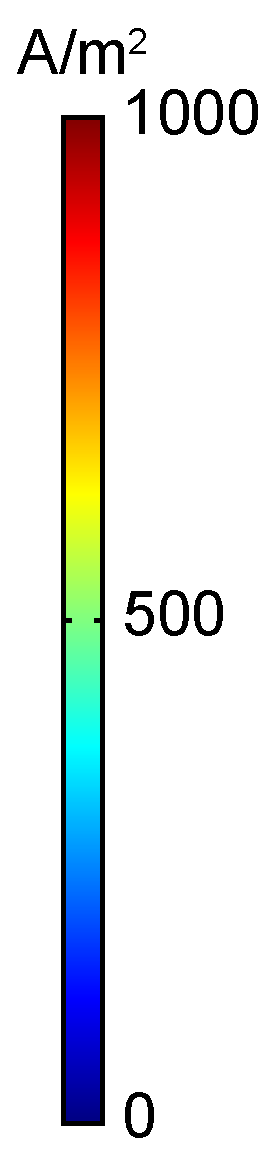
\includegraphics[height=5.3cm]{Validation/cbar_streamlines_short}
    \end{subfigure}%
    
    \caption[Streamline plots of the current paths during stimulation at
    E4]{Streamline plots of the current paths during stimulation at E4 for (a)
    grounding the nerve trunk, (b) grounding the caudal aspect of the temporal
    bone surface, (c) grounding or applying a 0.905 V offset on the temporal
    bone surface, (d) grounding the entire surrounding sphere, and (e) grounding
    at infinity. These correspond to the highlighted surfaces in
    Figure~\ref{fig:boundary_surfaces}. Scale indicates current density in the
    nerve tissue.}
	\label{fig:valid_streamlines}
\end{figure}

\subsection{Estimated Impact on Neural Excitation}

Differences in current flow pathways in turn affected predictions of neural
excitation as measured by the AF. The main regions of excitation were largely
similar for any particular stimulating electrode, but localised differences
along the neural sheet were also observed. Percentage differences in AF relative
to the base case (Figure~\ref{fig:unroll_neural_sheet}) are shown in
Figures~\ref{fig:valid_delta_af_TR} and \ref{fig:valid_delta_af_BC}. These plots
show the change in predicted AF at each node of Ranvier along the unrolled
neural sheet when a single simulation parameter was varied.

\begin{figure}
	\centering
	\hfill%
	\begin{subfigure}[t]{0.3\textwidth}
        \centering
        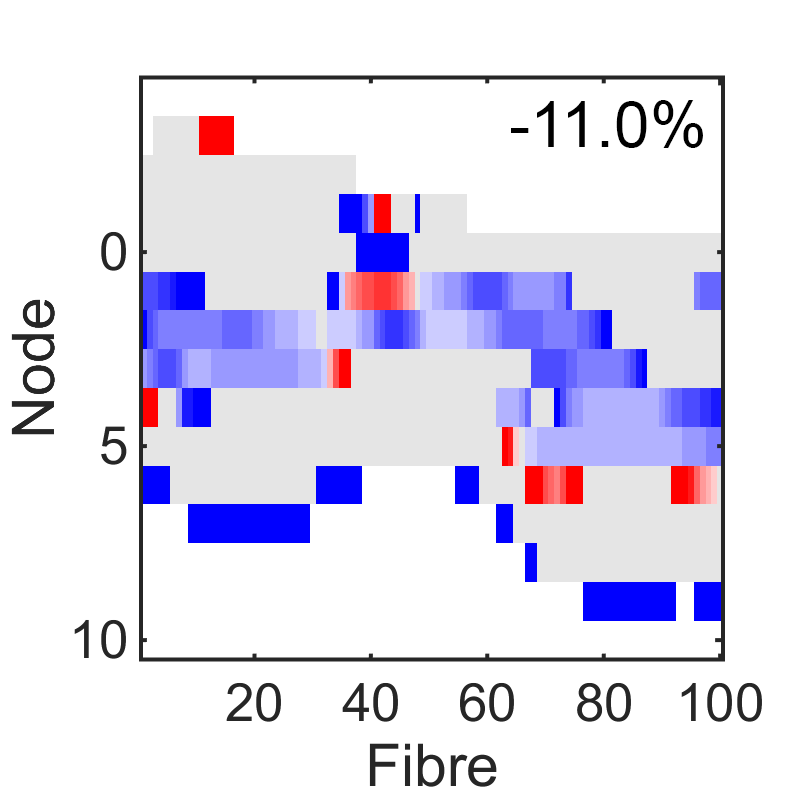
\includegraphics[height=4.5cm]{Validation/delta_af-TR-bone}
        \caption{Homogeneous bone}
        \label{fig:valid_delta_af_bone}
    \end{subfigure}%
	\begin{subfigure}[t]{0.3\textwidth}
        \centering
        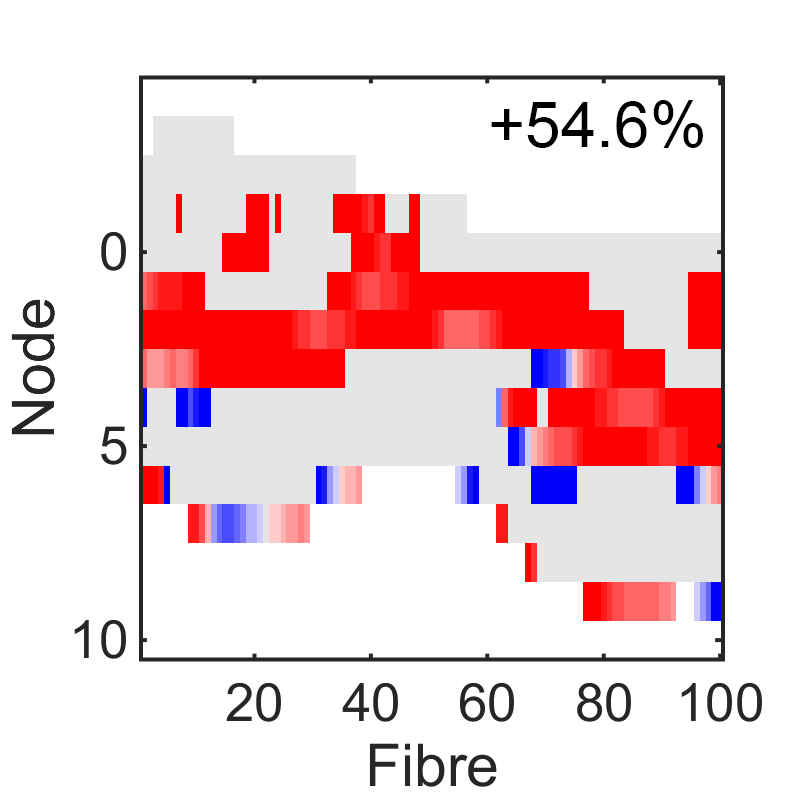
\includegraphics[height=4.5cm]{Validation/delta_af-TR-otic}
        \caption{Otic capsule}
        \label{fig:valid_delta_af_otic}
    \end{subfigure}%
	\begin{subfigure}[t]{0.3\textwidth}
        \centering
        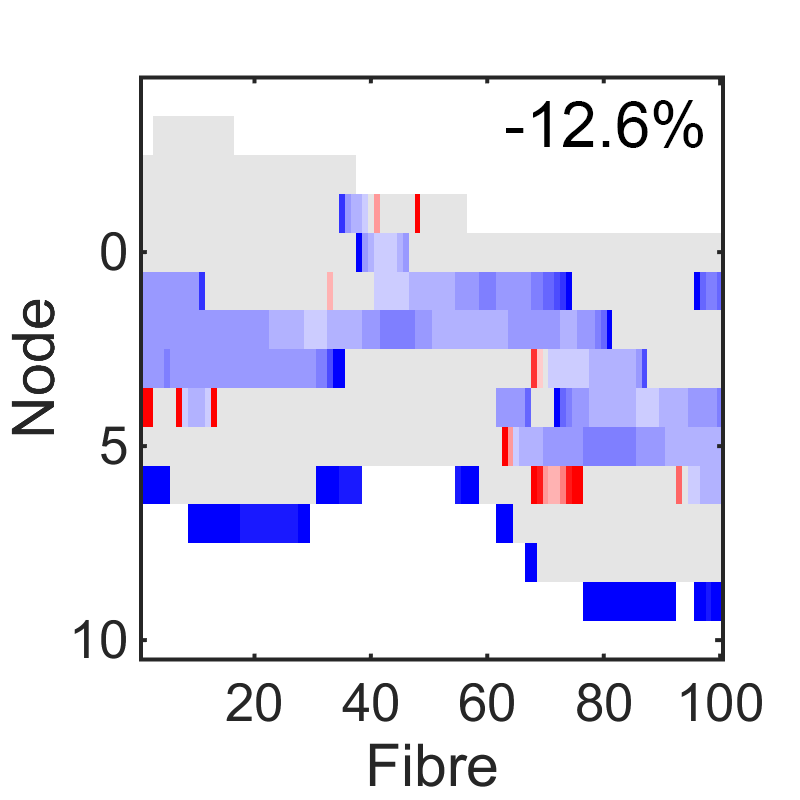
\includegraphics[height=4.5cm]{Validation/delta_af-TR-tempbone}
        \caption{Temporal bone}
        \label{fig:valid_delta_af_tempbone}
    \end{subfigure}%
    \begin{subfigure}[t]{0.09\textwidth}
        \centering
        \phantom{\hspace{1.4cm}}
    \end{subfigure}\\%
    \vspace{0.8em}%
    \hfill%
    \begin{subfigure}[t]{0.3\textwidth}
        \centering
        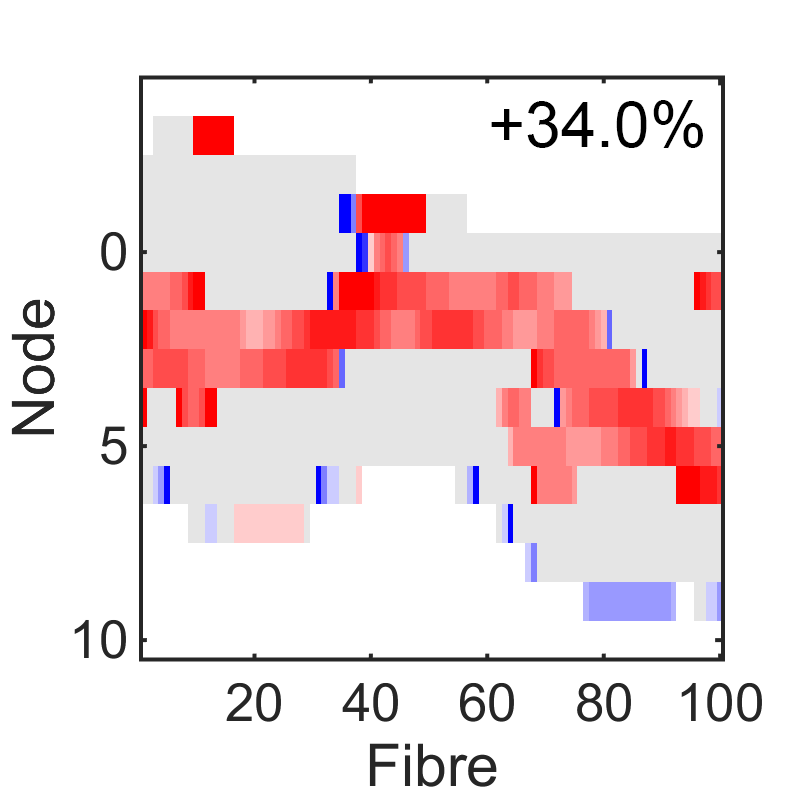
\includegraphics[height=4.5cm]{Validation/delta_af-TR-peri}
        \caption{Perilymph}
        \label{fig:valid_delta_af_peri}
    \end{subfigure}%
    \begin{subfigure}[t]{0.3\textwidth}
        \centering
        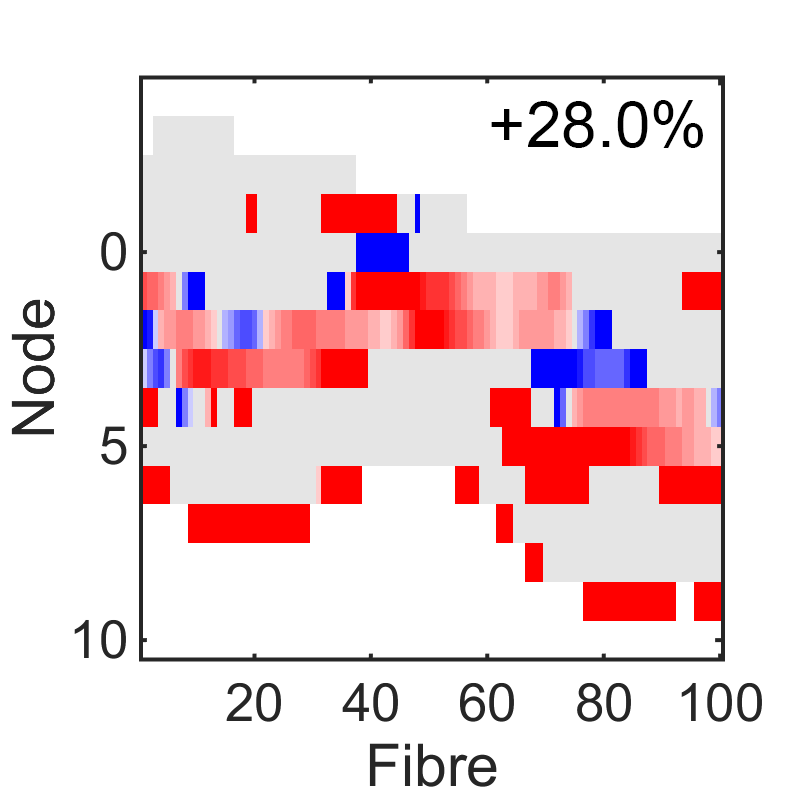
\includegraphics[height=4.5cm]{Validation/delta_af-TR-nerve}
        \caption{Nerve}
        \label{fig:valid_delta_af_nerve}
    \end{subfigure}%
    \begin{subfigure}[t]{0.3\textwidth}
        \centering
        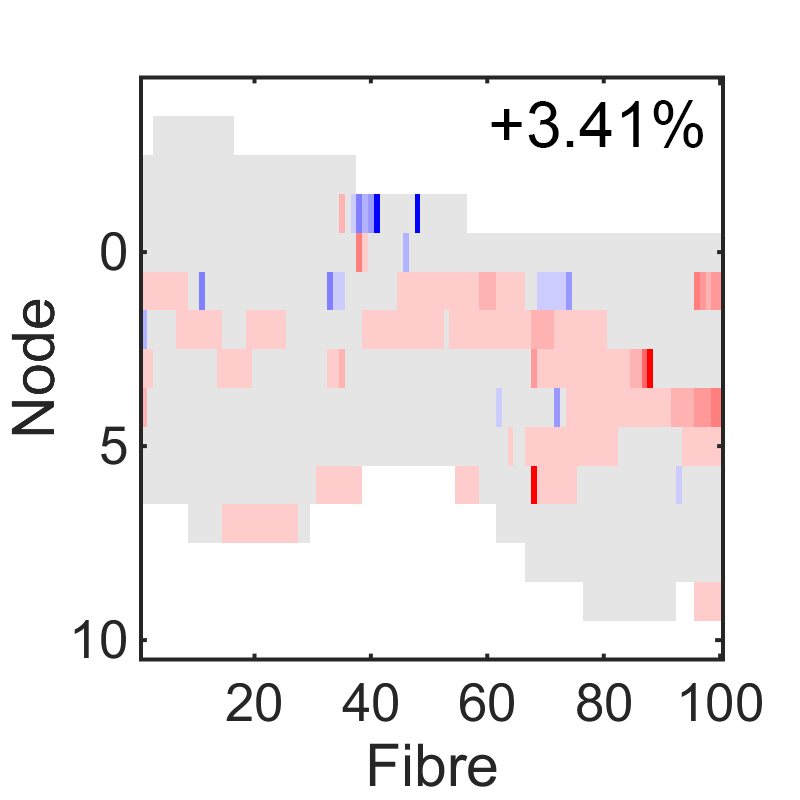
\includegraphics[height=4.5cm]{Validation/delta_af-TR-sl}
        \caption{Spiral ligament}
        \label{fig:valid_delta_af_sl}
    \end{subfigure}%
    \begin{subfigure}[t]{0.09\textwidth}
        \centering
        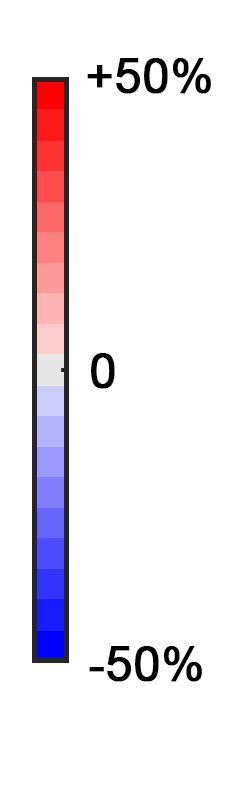
\includegraphics[height=4.5cm]{Validation/cbar_delta_af_short}
    \end{subfigure}%
    
    \caption[Percentage change in activating function with changes in tissue
    resistivity]{Percentage change in activating function with changes in tissue
    resistivity. Deltas were calculated relative to the base case. RMS deltas
    are shown in the top right corner. (Copyright \textcopyright{} 2015, IEEE.)}
	\label{fig:valid_delta_af_TR}
\end{figure}

\begin{figure}
	\centering
	
	\begin{subfigure}[t]{0.3\textwidth}
        \centering
        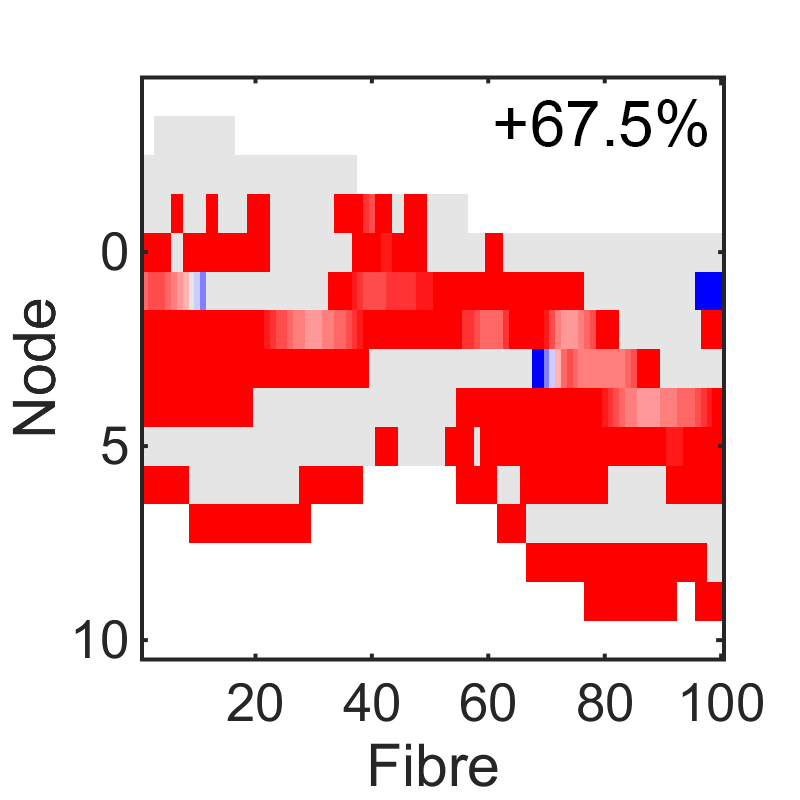
\includegraphics[height=4.5cm]{Validation/delta_af-BC-nerve}
        \caption{Nerve}
        \label{fig:valid_delta_af_nervetrunk}
    \end{subfigure}%
	\begin{subfigure}[t]{0.3\textwidth}
        \centering
        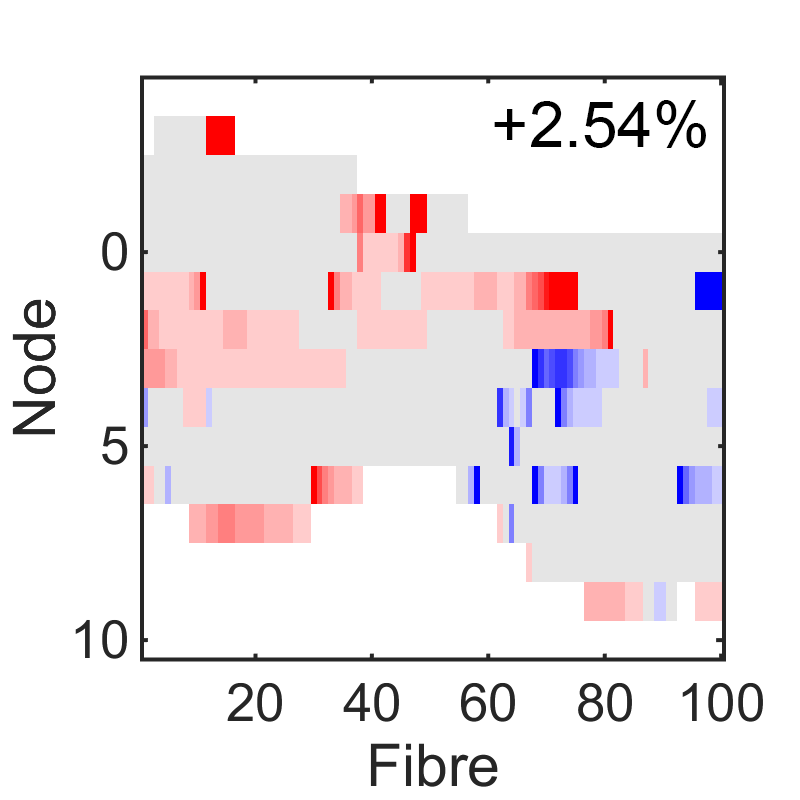
\includegraphics[height=4.5cm]{Validation/delta_af-BC-caud}
        \caption{Temporal bone (caudal)}
        \label{fig:valid_delta_af_caud}
    \end{subfigure}
	\begin{subfigure}[t]{0.3\textwidth}
        \centering
        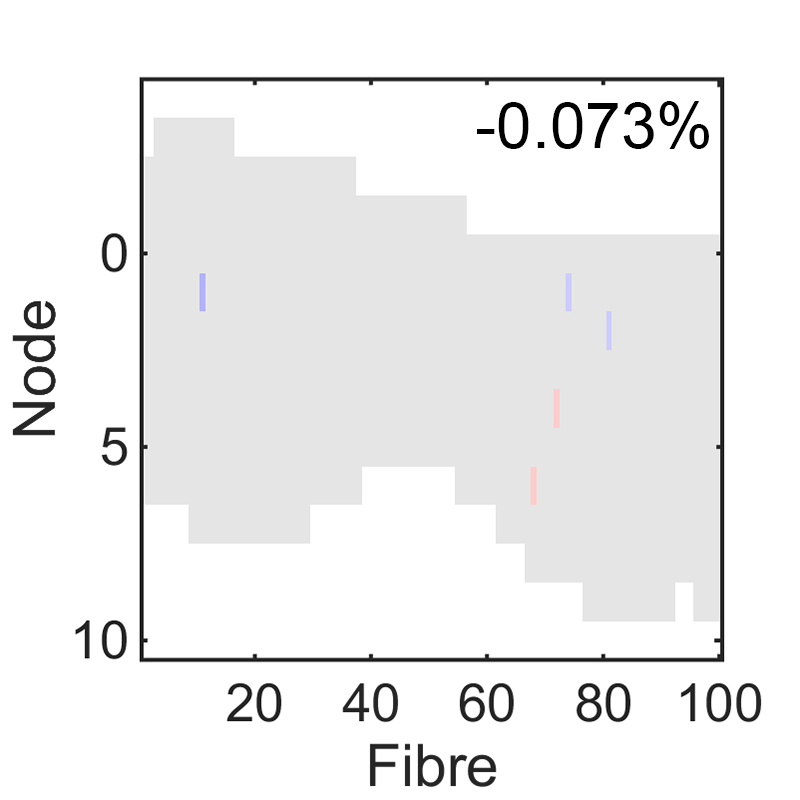
\includegraphics[height=4.5cm]{Validation/delta_af-BC-hemi_off}
        \caption{Temporal bone (offset)}
        \label{fig:valid_delta_af_hemioff}
    \end{subfigure}\\%
    \vspace{0.8em}\hspace{1cm}%
    \begin{subfigure}[t]{0.3\textwidth}
        \centering
        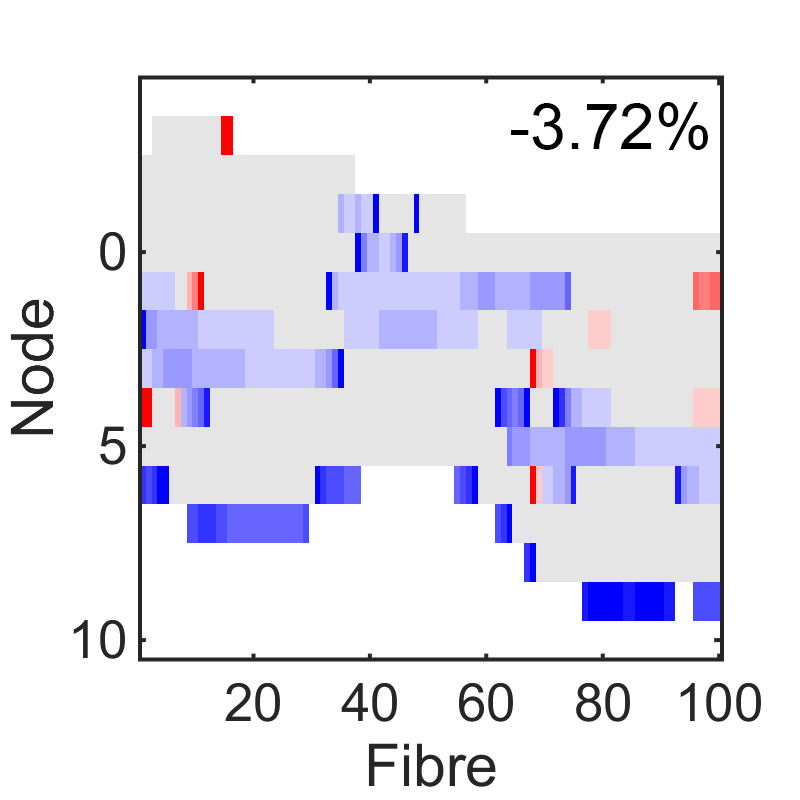
\includegraphics[height=4.5cm]{Validation/delta_af-BC-sph}
        \caption{Sphere}
        \label{fig:valid_delta_af_sph}
    \end{subfigure}%
    \begin{subfigure}[t]{0.3\textwidth}
        \centering
        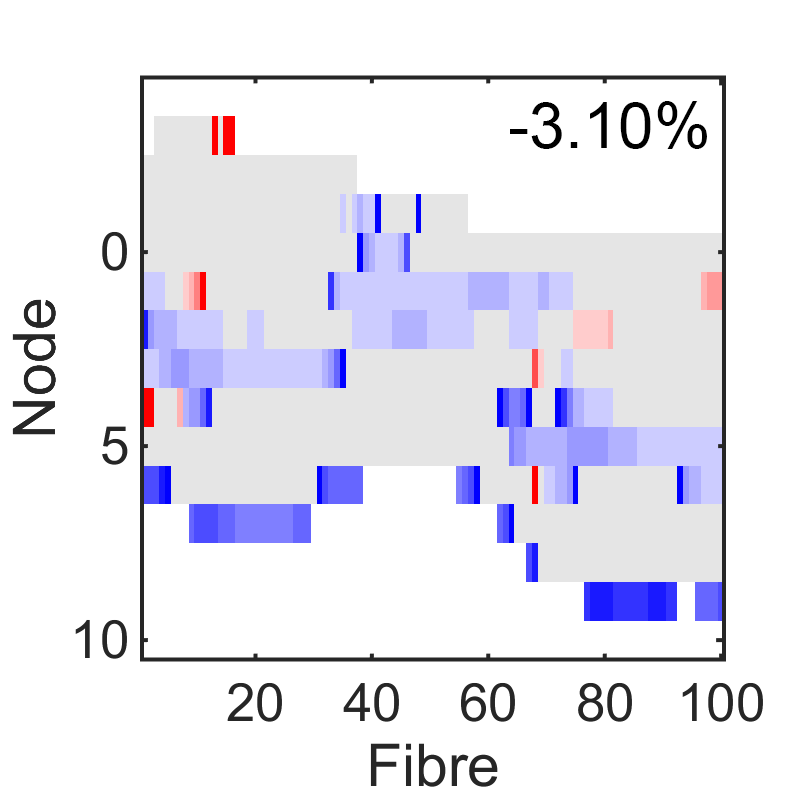
\includegraphics[height=4.5cm]{Validation/delta_af-BC-inf}
        \caption{Infinity}
        \label{fig:valid_delta_af_inf}
    \end{subfigure}%
    ~~%
    \begin{subfigure}[t]{0.09\textwidth}
        \centering
        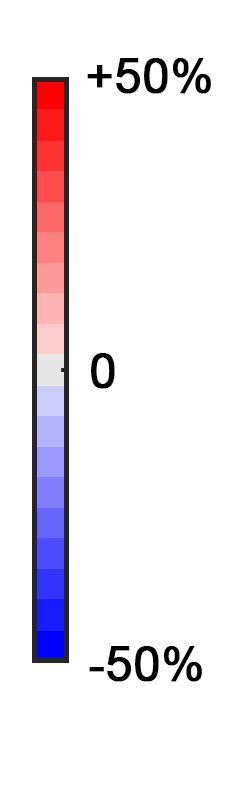
\includegraphics[height=4.5cm]{Validation/cbar_delta_af_short}
    \end{subfigure}%
    
    \caption[Percentage change in activating function with boundary
    conditions]{Percentage change in activating function with boundary
    conditions relative to the base case for (a) grounding the nerve trunk, (b)
    grounding the caudal aspect of the temporal bone surface, (c)
    applying a voltage offset to the temporal bone surface, (d) grounding the
    entire surrounding sphere, and (e) grounding at infinity. The voltage
    offset by itself had negligible effect on the AF prediction. (Copyright
    \textcopyright{} 2015, IEEE.)}
	\label{fig:valid_delta_af_BC}
\end{figure}

Figure~\ref{fig:valid_delta_af_bone}--\ref{fig:valid_delta_af_tempbone} show
that higher bone resistivity drove more current into the nerve tissue and
increased depolarisation relative to the base case, and vice versa. Likewise,
higher resistivities for perilymph, nerve, or the spiral ligament led to
increased axonal activity
(Figure~\ref{fig:valid_delta_af_peri}--\ref{fig:valid_delta_af_sl}). The
differences were not uniform and tended to be more pronounced near the main area
of excitation (especially at the peripheral process) as well as at fibres one
full turn away (around fibre 90).

For the boundary conditions, grounding the nerve trunk
(Figure~\ref{fig:valid_delta_af_nervetrunk}) resulted in significantly more
widespread depolarisation than in the other cases (+67.5\% RMS, the largest
discrepancy of all the test cases). The differences were largest near the end of
the axon where the ground was imposed. Grounding the caudal temporal bone
(Figure~\ref{fig:valid_delta_af_caud}) reflected the directionality of the
corresponding streamlines. AF values for the grounded temporal bone surface and
the corresponding offset case were virtually identical, which was expected given
their similar current pathways. A slightly larger discrepancy was observed
between the sphere grounding and infinite grounding conditions
(Figures~\ref{fig:valid_delta_af_sph} and \ref{fig:valid_delta_af_inf}).
Nonetheless, boundary conditions 2--6 all produced AF patterns that were within
about 5\% of each other, so the model was not sensitive to this assumption.

\section{Discussion}
\label{sect:validation_discussion}

\subsection{Modelling Workflow}

The methodology used in this study allowed for a high fidelity reconstruction of
the cochlea with an unprecedented amount of anatomical detail, but it also
suffered from a few drawbacks stemming from the large size of the data set.
Firstly, the time required to process the image stack was in the order of months
due to the large number of tissues and the need for some sophisticated manual
segmentation. Secondly, the segmentation process required comprehensive
knowledge of the anatomy in the region of interest, and consultations with
anatomical experts were needed to minimise the risk of incorrect reconstruction.
Algorithmic segmentation could be employed in the future to reduce the time
requirements and inconsistencies due to human error, but to the extent of the
authors' knowledge, existing techniques are not well suited to datasets with
many tissues and are usually optimised for CT or MRI image stacks. Thirdly,
although the Octree algorithm was robust enough to handle the complexity of the
surfaces, it always resulted in the production of some small element islands.
While smoothing the segmentation eliminated some of these islands, the
requirement for manual intervention limits the potential for a fully automated
process.

Overall, the capabilities of this workflow far outweighed its limitations. It
can be expected to translate well to other data-sets and other organs,
regardless of imaging modality.

\subsection{Material Properties}

There is some concern that the base resistivity values for cochlear-specific
tissues may not be appropriate because the scaling and disregard of spatial
effects necessary to derive them from bulk resistances compromises their
accuracy\cite{girzon1987,finley1990,frijns1995,micco2006}. Most values can also
be traced back to a single source~\cite{strelioff1973}, so there is doubt over
the reliability of the measurements.

According to the simulation results, the model is not very sensitive to most
tissue resistivities. The spread of terminal voltage predictions in
Figure~\ref{fig:voltage_sensitivity_TR} is smaller than the standard deviation
of the \invivo{} measurements, suggesting that any uncertainties were within
inter-subject variability limits. The continued use of these values in the
literature also suggests that they represent the electric behavior reasonably
well.

For the tissues to which the model was sensitive, some (namely CSF, endolymph,
and perilymph) have resistivities that are known
accurately~\cite{frijns1995,gabriel2009} and can therefore be used with
confidence. The FE model in this study was based on a healthy, unimplanted
guinea pig cochlea, and the validation data was obtained from acute experiments,
so the base value of perilymph resistivity was suitable. In chronic implants
however, the perilymph around the electrode array is displaced by a layer of
fibrous encapsulation tissue~\cite{grill1994}. Given the sensitivity of the
model to perilymph resistivity, this would have a bearing on predictions of
stimulation thresholds~\cite{hanekom2005}.

Terminal voltages were most sensitive to the bone domains because injected
current must pass through them to reach ground. As such, these values were
particularly crucial. The Suesserman resistivity
measurements~\cite{suesserman1992} used in this study are specific to the guinea
pig and, given the care with which they were taken, should be quite accurate.
However, it is curious that the lateral wall was reported as being less
resistive than the modiolar wall because higher density bone is more
resistive~\cite{williams1996} and the otic capsule is the densest bone in the
body~\cite{bast1949}. The use of the skull value for the temporal bone and
infinite domains may also be an underestimate since the temporal bone is
relatively dense. Conversely, the current path through the head is likely to
follow lower resistance pathways, such as through the CSF~\cite{tran2015}.
Determining the true effect on the return pathway would require a whole head
model.

The resistivity of the spiral ligament should also be verified. At 0.6~$ \Omega
\cdot $m, it is relatively low, reflecting the suspicion that perilymph can
diffuse freely through it and that it is involved in ion
transport~\cite{dallos1996,slepecky1996}. However, considering the known
presence of various cell types and extracellular matrix material in the tissue,
and that perilymph itself has a resistivity of 0.7~$ \Omega \cdot $m, this may
be inaccurate. The only other estimate in the literature is 2.5~$ \Omega \cdot
$m~\cite{girzon1987}. At this higher resistivity, the scala media became more
insulated, leading to differences in terminal voltages, current pathways, and
AF. It may be worth investigating whether the scala media should be modelled as
being insulated on all sides to represent the tight junctions between the
surrounding epithelial cells that prevent ionic current flow
\invivo{}~\cite{dallos1996}.

The ideal resolution to these uncertainties over material properties would be to
re-measure the resistivities of all the cochlear tissues using an accurate and
up-to-date technique~\cite{spelman1990}. At the least, this would provide an
alternative data point for comparison with the values derived from
lumped-element models; at best, these values would form a new gold standard as
inputs for future electroanatomical studies of the cochlea.

\subsection{Boundary Conditions}
\label{sect:valid_bc_discussion}

Three criteria were considered for evaluating the boundary conditions: closeness
of match to the \invivo{} terminal voltages
(Figure~\ref{fig:voltage_sensitivity_BC}), the current paths exiting the cochlea
(Figure~\ref{fig:valid_streamlines}), and the impact on AF values
(Figures~\ref{fig:valid_delta_af_TR} and \ref{fig:valid_delta_af_BC}).

Grounding the nerve trunk seemed to make sense based on early evidence that the
nerve trunk is the dominant exit pathway~\cite{vonbekesy1960}. Using this
boundary condition, simulated voltages were relatively high because current was
forced to flow through a small return area. However, the otic capsule is not a
perfect insulator and both the stimulating and return electrodes are small
relative to the head, so injected current spreads out as it flows through the
cochlear tissues and is not expected to re-converge within the
domain~\cite{baker1989,tran2015} as observed in
Figure~\ref{fig:valid_streams_nerve}. Because of this, the AF plot
(Figure~\ref{fig:valid_delta_af_nervetrunk}) predicted substantially more
widespread depolarization than the other boundary conditions. Combined with the
relative proximity of this isosurface to the regions of interest within the
domain, it appears that this boundary condition violates Saint-Venant's
Principle of far field equivalence by not faithfully reproducing true MP loading
patterns. The evidence suggests that grounding the end of the modelled nerve
trunk is inappropriate, at least in the case of the guinea pig cochlea.

Simply grounding an outer surface to represent the current sink is also
insufficient. It ignores the presence of the return path through the head and
thus underestimates intrascalar voltages. Including the return path as an
infinite domain is plausible, but tends to overestimate voltages. Of course,
this depends on the resistivity of the infinite domain, and a value could be
applied that forces a match with the \invivo{} data, but that would alter the
ratio of resistivities between the temporal bone and other cochlear tissues,
which could result in unintended effects on the current paths within the
cochlea~\cite{micco2006,wong2013mb} and the AF (e.g.
Figure~\ref{fig:valid_delta_af_otic}). This is not ideal because resistivities
are not a variable and can be measured. The value used for the infinite element
domain in this study appears to be higher than the effective resistivity of the
mean guinea pig head. In any case, purely grounded boundary conditions cannot be
easily matched to \invivo{} data, which may be important in future
subject-specific modeling efforts.

Given that none of the above boundary conditions presented a close match to the
\invivo{} data, the voltage offset was proposed and tested. This alternative
explanation for the voltage drop along the unmodelled return path through the
head did not seem to influence the current pathways or AF, presumably because it
is cancelled out in the calculation. Its value could therefore be set
arbitrarily to model different cases, as required for subject-specific models.
The principle could also be applied to cochlear models from other species.

The offset would ideally be applied to a grounding surface that replicates the
\invivo{} current paths. In these simulations, grounding the temporal bone
surface was considered to be the most realistic because the protrusion of the
guinea pig cochlea into the tympanic bulla, the low voltages exhibited during CI
stimulation, and the extremely high impedance of air together suggested that
injected current would flow away from the bulla
(Figure~\ref{fig:valid_streams_hemi}). However, there is no way to be sure
without implementing a complete guinea pig head model.

Ultimately, grounding surfaces need to be sufficiently large and far from the
stimulating electrode in models of MP stimulation to prevent adverse impacts on
the computed AF.

\subsection{Study Limitations}

The trajectory of the electrode array within the scala tympani was unlikely to
be a perfect match despite taking care to accurately replicate the insertion at
the round window. HL8 arrays tend towards a more lateral position, but the exact
\invivo{} positions of each electrode were not confirmed in this study. Each
insertion was also slightly different, and the data for more apical stimulation
suggest that the modelled insertion was slightly deeper than the \invivo{}
average. This adds a little uncertainty to the \insilico{} predictions, but the
close fit inspires confidence in the model nonetheless.

Another concern was that the \invivo{} measurements were taken at the end of the
stimulating phase. It is known that the voltage profile changes over the
duration of the pulse, and there is some speculation that time-dependent effects
may play a role despite Spelman's observations~\cite{spelman1982}. Until this
hypothesis is tested, the purely resistive formulation of this model should only
be taken as a first approximation.

Lastly, the sample size for the \invivo{} measurements was relatively small.
Ideally, more measurements would be added to the comparison, not only from more
animals, but also from more locations within each animal to validate the field
quantities outside the scala tympani. However, this must be balanced against the
financial, time, and ethical costs of obtaining these additional data points. It
is hoped that if \insilico{} models such as the one presented here become
sufficiently accurate and trustworthy, the reliance on animal testing may be
reduced in the long term.

\section{Conclusions}

The workflow used in this study successfully overcame the difficulties seen in
other \insilico{} modeling methodologies to enable the creation of a high
fidelity FE model of the guinea pig cochlea. Intrascalar voltages predicted by
the model were more sensitive to the choice of boundary condition than to the
assigned tissue resistivity values. However, the AF along the neural sheet was
more sensitive to certain material properties. Grounding the nerve trunk
appeared to be inappropriate for the guinea pig model; conversely, the proposed
voltage offset boundary condition was able to characterise multiple facets of
the \invivo{} situation realistically. In addition, the offset provides a
feasible method for accommodating subject-specific differences, and may
therefore be considered for use in future models of monopolar CI stimulation.

Overall, the strong correlation between the \insilico{} results and the average
\invivo{} measurements indicated that the model can be used to represent an
average implanted guinea pig cochlea.
